%  LaTeX support: latex@mdpi.com 
%  For support, please attach all files needed for compiling as well as the log file, and specify your operating system, LaTeX version, and LaTeX editor.

%=================================================================
\documentclass[physics,article,accept,pdftex,moreauthors]{Definitions/mdpi} 
% For posting an early version of this manuscript as a preprint, you may use "preprints" as the journal and change "submit" to "accept". The document class line would be, e.g., \documentclass[preprints,article,accept,moreauthors,pdftex]{mdpi}. This is especially recommended for submission to arXiv, where line numbers should be removed before posting. For preprints.org, the editorial staff will make this change immediately prior to posting.

%--------------------
% Class Options:
%--------------------
%----------
% journal
%----------
% Choose between the following MDPI journals:
%  physics 

%---------
% article
%---------
% The default type of manuscript is "article", but can be replaced by: 
% abstract, addendum, article, book, bookreview, briefreport, casereport, comment, commentary, communication, conferenceproceedings, correction, conferencereport, entry, expressionofconcern, extendedabstract, datadescriptor, editorial, essay, erratum, hypothesis, interestingimage, obituary, opinion, projectreport, reply, retraction, review, perspective, protocol, shortnote, studyprotocol, systematicreview, supfile, technicalnote, viewpoint, guidelines, registeredreport, tutorial
% supfile = supplementary materials

%----------
% submit
%----------
% The class option "submit" will be changed to "accept" by the Editorial Office when the paper is accepted. This will only make changes to the frontpage (e.g., the logo of the journal will get visible), the headings, and the copyright information. Furthermore, line numbering will be removed. Journal info and pagination for accepted papers will also be assigned by the Editorial Office.

%------------------
% moreauthors
%------------------
% If there is only one author the class option oneauthor should be used. Otherwise use the class option moreauthors.

%---------
% pdftex
%---------
% The option pdftex is for use with pdfLaTeX. If eps figures are used, remove the option pdftex and use LaTeX and dvi2pdf.

%=================================================================
% MDPI internal commands - do not modify
\firstpage{1} 
\makeatletter 
\setcounter{page}{\@firstpage} 
\makeatother
\pubvolume{1}
\issuenum{1}
\articlenumber{0}
\pubyear{2023}
\copyrightyear{2023}
%ae
\datereceived{26 December 2022} 
\daterevised{17 March 2023} % Comment out if no revised date
\dateaccepted{23 March 2023} 
\datepublished{ } 
%\datecorrected{} % For corrected papers: "Corrected: XXX" date in the original paper.
%\dateretracted{} % For corrected papers: "Retracted: XXX" date in the original paper.
\hreflink{https://doi.org/} % If needed use \linebreak
%\doinum{}
%\pdfoutput=1 % Uncommented for upload to arXiv.org

%=================================================================
% Add packages and commands here. The following packages are loaded in our class file: fontenc, inputenc, calc, indentfirst, fancyhdr, graphicx, epstopdf, lastpage, ifthen, lineno, float, amsmath, setspace, enumitem, mathpazo, booktabs, titlesec, etoolbox, tabto, xcolor, soul, multirow, microtype, tikz, totcount, changepage, attrib, upgreek, cleveref, amsthm, hyphenat, natbib, hyperref, footmisc, url, geometry, newfloat, caption

\newcommand{\aap}{{\it Astron. Astrophys.}}
\newcommand{\aaps}{{\it Astron. Astrophys. Suppl.}}
\newcommand{\apj}{{\it Astrophys. J.}}
\newcommand{\apjl}{{\it Astrophys. J. Lett.}}
\newcommand{\apss}{{\it Astrophys. Space Sci.}} 
\newcommand{\solphys}{{\it Sol. Phys.}}
\newcommand{\ssr}{{\it Space Sci. Rev.}}
%=================================================================
%% Please use the following mathematics environments: Theorem, Lemma, Corollary, Proposition, Characterization, Property, Problem, Example, ExamplesandDefinitions, Hypothesis, Remark, Definition, Notation, Assumption
%% For proofs, please use the proof environment (the amsthm package is loaded by the MDPI class).

%=================================================================
% Full title of the paper (Capitalized)
\Title{\highlighting{$p$}%MDPI:Please use a consistent style for the letters throughout the paper, (e.g., italic or not).
-Mode Oscillations in Highly Gravitationally Stratified Magnetic Solar Atmospheres}

% MDPI internal command: Title for citation in the left column
\TitleCitation{\hl{p}-Mode Oscillations in Highly Gravitationally Stratified Magnetic Solar Atmospheres}

% Author Orchid ID: enter ID or remove command
\newcommand{\orcidauthorA}{0000-0002-4055-2315}
\newcommand{\orcidauthorB}{0000-0002-0049-4798}
\newcommand{\orcidauthorC}{0000-0003-3439-4127}
% Add \orcidA{} behind the author's name
%\newcommand{\orcidauthorB}{0000-0000-0000-000X} % Add \orcidB{} behind the author's name

% Authors, for the paper (add full first names)
%\Author{Michael Griffiths $^{1,\dagger,\ddagger}$\orcidA{}, Robertus Erd\'{e}lyi %$^{2,\ddagger}$, Ruisheng Zheng $^{3,}$* and Norbert Gyenge $^{4,}$*}

\Author{\hl{Michael Griffiths} %MDPI: Please carefully check the accuracy of names and affiliations.
 $^{1,}$*\orcidA{}, Norbert Gyenge $^{1,\highlighting{2}%MDPI: 1. The affiliation numbers should appear in numerical order. Please check the suggested changes. 2. Duplicate affiliations information should be merged in one item, the list number needs to be changed at the same time, Please check the changes.
}$, Ruisheng Zheng $^{3}$, Marianna Korsós $^{1,4,5,6}$\orcidB{} \linebreak and Robertus Erd\'{e}lyi $^{1,5,6}$\orcidC{}}


%\longauthorlist{yes}

% MDPI internal command: Authors, for metadata in PDF
\AuthorNames{Michael Griffiths, Norbert Gyenge, Ruisheng Zheng, Marianna Korsós and Robertus Erd\'{e}lyi}

% MDPI internal command: Authors, for citation in the left column
\AuthorCitation{Griffiths, M.; Gyenge, N.R.; Zheng, R.; Korsós, M; Erd\'{e}lyi, R.}
% If this is a Chicago style journal: Lastname, Firstname, Firstname Lastname, and Firstname Lastname.

% Affiliations / Addresses (Add [1] after \address if there is only one affiliation.)
\address{%
$^{1}$ \quad Research IT, The University of Sheffield, 10-12 Brunswick Street, Sheffield S10 2FN, UK; n.g.gyenge@sheffield.ac.uk (N.G.); marianna.korsos@dfa.unict.it (M.K.); robertus@sheffield.ac.uk (R.E.)\\
$^{2}$ \quad Hungarian Solar Physics Foundation (HSPF), Pet\H{o}fi t\'er 3, \hl{H-}%MDPI: Please confirm whether this is part of the post code, can it be deleted?
5700 Gyula, Hungary\\
$^{3}$ \quad Shandong Key Laboratory of Optical Astronomy and Solar-Terrestrial Environment, School of Space Science and Physics, Institute of Space Sciences, Shandong University, Weihai 264209, China; ruishengzheng@sdu.edu.cn\\
$^{4}$ \quad Dipartimento di Fisica e Astronomia ``Ettore Majorana", Universit\`a di Catania, Via S. Sofia 78, \hl{I}~%MDPI: Please confirm whether this is part of the post code, can it be deleted? MKG Yes it can be deleted
95123~Catania,~Italy\\
$^{5}$ \quad Deptartment of Astronomy, E\"otv\"os L. University, P\'azm\'any P\'eter s\'et\'any 1/a, \hl{H-}1117 Budapest, Hungary\\
$^{6}$ \quad Solar Physics and Space Plasma Research Centre ($SP^{2}RC$), School of Mathematics and Statistics, University~of~Sheffield, Hicks Building, Hounsfield Road, \hl{Sheffield S3 7RH}%MDPI: We added city and revised post code by google, please confirm. MKG Confirmed
, UK
}


% Contact information of the corresponding author
\corres{Correspondence: m.griffiths@sheffield.ac.uk}

% Current address and/or shared authorship
%\firstnote{Current address: Affiliation 3.} 
%\secondnote{These authors contributed equally to this work.}
% The commands \thirdnote{} till \eighthnote{} are available for further notes

%\simplesumm{} % Simple summary

%\conference{} % An extended version of a conference paper


%FIXME - THIS COMMENT WILL BE REMOVED WHEN A FIX COMPLETED REPLACED WITH UPDATE E.G. SEE BELOW


%FIXME IMPROVE CAPTIONS FOR FIGURES



% Abstract (Do not insert blank lines, i.e., \\) 

 
\abstract{The aim of the 
 %work 
\highlighting{study} %MDPI: "study", "paper", "investigation", "revoiiew" instead of "work", "article", "manuscript" etc. recommended for scientific papers. Please consider. Here and elsewhere below.
reported in this paper is to gain understanding of solar global oscillations and the propagation characteristics of $p$-mode oscillations in the highly gravitationally stratified magnetic solar atmosphere. The paper presents the results of 
 \highlighting{3D (3-dimensional)} %MDPI: No undefined abbreviations, variables, notations, indexes ets. when first met in abstract, maintext, figures, tables. 
numerical magnetohydrodynamic (MHD) simulations of a model solar atmosphere with a uniform, vertical and cylindrically symmetric magnetic field. We use simulation drivers which result in oscillations  mimicking the behaviour of $p$-mode oscillations. The paper reports the variation of the energy flux and oscillation frequency of the magnetosonic modes and examines their dependence on the magnetic field strength.  We report results for the temporal analysis of observational data for the 
\highlighting{quiet 
 %Quiet
} %MDPI: is the capital letter necessary? Moreover used also the lower-case below. Suggested the lower-case always. Here and through the paper.   
Sun and for a region containing a small sunspot (solar pore). We compare the temporal analysis of results from observations of these ubiquitous intensity oscillations with numerical simulations of potential signatures of global oscillations of the solar atmosphere.  We conclude that magnetic regions of the solar atmosphere are favourable regions for the propagation of a small leakage of energy by slow magnetosonic modes. The results also exhibit a variation in the frequency  of the oscillations at different heights in the low-to-mid solar atmosphere and for different values of the magnetic field. The  numerically obtained periodic behaviour and variation in frequency, even in this simplified model atmosphere, is consistent with the observational data. We find frequencies and frequency variations that are similar to measurements obtained from the intensity time series of images taken by the Solar Dynamics Observatory.}

% Keywords
\keyword{MHD, \highlighting{$p$}-mode, magnetic, solar, atmosphere} 

% The fields PACS, MSC, and JEL may be left empty or commented out if not applicable
%\PACS{J0101}
%\MSC{}
%\JEL{}

%%%%%%%%%%%%%%%%%%%%%%%%%%%%%%%%%%%%%%%%%%
% Only for the journal Diversity
%\LSID{\url{http://}}

%%%%%%%%%%%%%%%%%%%%%%%%%%%%%%%%%%%%%%%%%%
% Only for the journal Applied Sciences
%\featuredapplication{Authors are encouraged to provide a concise description of the specific application or a potential application of the work. This section is not mandatory.}
%%%%%%%%%%%%%%%%%%%%%%%%%%%%%%%%%%%%%%%%%%

%%%%%%%%%%%%%%%%%%%%%%%%%%%%%%%%%%%%%%%%%%
% Only for the journal Data
%\dataset{DOI number or link to the deposited data set if the data set is published separately. If the data set shall be published as a supplement to this paper, this field will be filled by the journal editors. In this case, please submit the data set as a supplement.}
%\datasetlicense{License under which the data set is made available (CC0, CC-BY, CC-BY-SA, CC-BY-NC, etc.)}

%%%%%%%%%%%%%%%%%%%%%%%%%%%%%%%%%%%%%%%%%%
% Only for the journal Toxins
%\keycontribution{The breakthroughs or highlights of the manuscript. Authors can write one or two sentences to describe the most important part of the paper.}

%%%%%%%%%%%%%%%%%%%%%%%%%%%%%%%%%%%%%%%%%%
% Only for the journal Encyclopedia
%\encyclopediadef{For entry manuscripts only: please provide a brief overview of the entry title instead of an abstract.}

%%%%%%%%%%%%%%%%%%%%%%%%%%%%%%%%%%%%%%%%%%
% Only for the journal Advances in Respiratory Medicine
%\addhighlights{yes}
%\renewcommand{\addhighlights}{%

%\noindent This is an obligatory section in “Advances in Respiratory Medicine”, whose goal is to increase the discoverability and readability of the article via search engines and other scholars. Highlights should not be a copy of the abstract, but a simple text allowing the reader to quickly and simplified find out what the article is about and what can be cited from it. Each of these parts should be devoted up to 2~bullet points.\vspace{3pt}\\
%\textbf{What are the main findings?}
% \begin{itemize}[labelsep=2.5mm,topsep=-3pt]
% \item First bullet.
% \item Second bullet.
% \end{itemize}\vspace{3pt}
%\textbf{What is the implication of the main finding?}
% \begin{itemize}[labelsep=2.5mm,topsep=-3pt]
% \item First bullet.
% \item Second bullet.
% \end{itemize}
%}

%%%%%%%%%%%%%%%%%%%%%%%%%%%%%%%%%%%%%%%%%%
\begin{document}

%%%%%%%%%%%%%%%%%%%%%%%%%%%%%%%%%%%%%%%%%%
%\setcounter{section} %% Remove this when starting to work on the template.
%\endnote{This is an endnote.} % To use endnotes, please un-comment \printendnotes below (before References). Only journal Laws uses \footnote.
% The order of the section titles is different for some journals. Please refer to the "Instructions for Authors” on the journal homepage.

\section{Introduction}

Theoretical and computational studies coupled with observations from solar telescopes,  both from ground or space, reveal diverse structures and dynamics in the Sun's atmosphere. The~culmination of these studies of the  chromosphere and the upper solar atmosphere has enhanced our knowledge of the variety of magnetic field structures.  Despite our armoury of observations and the diverse range of computational models, it still remains a challenge to make sense of this complex menagerie of dynamic structures to understand solar atmospheric heating (i.e., chromospheric and coronal) and more generally, space weather~phenomena.


An example of the dynamical complexity are the ubiquitous five-minute oscillations in the  lower solar atmosphere  (i.e., in~particular in the photosphere) that are referred to as the solar global acoustic oscillations or $p$-modes. These global oscillations are interpreted as trapped acoustic waves, i.e.,~standing acoustic oscillations of the solar interior. Earlier models of these oscillations assumed that there was reflection by the photosphere with at most some small evanescent propagation above the photosphere. The~$p$-modes were interpreted as resonant modes trapped in a cavity formed from the steep change in density at the solar surface and a lower turning point in the interior caused by the increase in the speed of sound resulting in refraction. The~physical characteristics of the solar sub-surface layers can be estimated using observations of the standing modes.  There is now increasing evidence for leakage of these modes. %The complexity and variety of magnetic structures in the solar atmosphere  give rise to a mixture of waves providing powerful diagnostics to aid our understanding and advance our knowledge  about these~structures.

   


%FIXME
%EXPLAIN IMPORTANCCE OF GLOBAL VERSUS LOCAL PHENOMENA HIGHLIGHT IN PAPER WHAT IS THE IMPORTANCE OF THE COUPLED ATMOSPHERE
%UPDATE
 The photosphere, chromosphere and transition layer act as a boundary layer coupling the solar interior and the solar corona. The~frequency shifts of global oscillations resulting  from boundary layers   and the influence of the coupling of the internal oscillations with the solar atmosphere have been investigated; see, e.g.,~the review~\cite{Erdelyi2006}.  A~number of earlier studies addressed the link between oscillations in the solar atmosphere and solar global oscillations;  this is also the topic of the computational modelling 
 %work 
\hl{study} 
described in this paper. An~outward propagating wave is reflected inward from the lower solar atmosphere, or~boundary layer, because~of a sudden decrease in the plasma density, while the lower boundary of the cavity is formed by the increasing sound speed due to temperature rises. For~global oscillation modes that exceed the acoustic cut-off frequency, there is wave leakage out from the cavity into the atmosphere. An~analytical model for understanding the behaviour of solar global oscillations based on the Klein--Gordon equation has been  developed~\cite{Taroyan2008}. This model suggests a global resonance. Waves  that are normally trapped by a frequency cut-off barrier are enhanced by a resonance enabling propagation into the upper solar atmosphere. The~inhomogeneous three-layer model leads to characteristic frequencies. Further work resulted in enhancements to the models described earlier~\cite{Pinter2007}.  This work utilised an exponentially decaying horizontal magnetic field as a representation of the magnetic carpet.  The~influence of the chromosphere-transition-corona boundary, the~relationship between magnetic structures and velocity wave perturbations had been the subject of a number of observational studies~\cite{Mein1976,Schmieder1980}. Some of these results indicate that small amounts of energy would propagate but that shock heating was unlikely to be a major source of coronal heating. Such studies were focused on the localised phenomena rather than on the global nature of the atmospheric~oscillations.
 
 For a number of decades, oscillations in the solar atmosphere have been the subject of observation and study, e.g.,~the reviews~\cite{Banerjee2011,deMoortel2009,Mathioudakis2013,Ruderman2009,Wang2011}. The~observed periods of atmospheric intensity oscillations range from  a few seconds to several hours~\cite{Auchere2014}. Much earlier, it was proposed by~\cite{Jensen1963}, that the 3- and 5-minute oscillations were the characteristics of the photosphere and the chromosphere. Recently, the~association of intensity oscillations with oscillations in coronal loops and sunspots has been confirmed for oscillation periods of three minutes. The~application of solar magneto-seismology (SMS) to intensity observations in the solar atmosphere can be used to understand the magnetic structures in the solar atmosphere, see, e.g.,~\cite{Roberts1984,Banerjee2007,Zaqarashvili2007,Erdelyi2008,Verth2010}.  Evidence for global oscillations  in the chromosphere and corona is suggested by the observational analysis of~\cite{Gyenge2018},  which demonstrates the frequent recurrence of micro-flare events with fluctuations between 3 min and 12 min. These fluctuations arise during time intervals before and after major solar~flares.


The key point of this %work
 \hl{study}  
is a comparison of numerical simulations  of a simplified solar atmosphere with observations, searching for a  potential link between ubiquitous upper atmospheric oscillations and the global solar oscillations. We use a  simple numerical representation that is of sufficient complexity to reveal the dominant dynamical processes in the magnetic solar atmosphere. Comparison of the reported observational work with the results of the modelling provides an indication that the modelling is sufficiently complex to give an insight into the physical mechanisms behind the behaviour of solar global oscillations. We report the results of numerical simulations of photospheric $p$-mode oscillations in a model solar atmosphere with a uniform and vertical magnetic field. We also present the results of a temporal analysis based on observations of intensity oscillations with the objective of providing evidence of the existence of the temporal behaviour exhibited by our simulations. The~work contributes to our understanding of the propagation and modification of global oscillations in the highly gravitationally stratified solar~atmosphere. 




%%%%%%%%%%%%%%%%%%%%%%%%%%%%%%%%%%%%%%%%%%




%%%%%%%%%%%%%%%%%%%%%%%%%%%%%%%%%%%%%%%%%%
\section{Motivation}\label{sec2}
\label{sec:motivation}

Given the complexity of the dynamics and the diversity of structures in the solar atmosphere, it is understood that a truly realistic model is challenging and  requires a hybrid multi-disciplined approach. Many computational 
 \hl{magnetohydrodynamic (MHD)}  
simulations of the Sun have been undertaken, some of the approaches have resulted in an encouraging degree of realism~\cite{Vogler2005,Gudiksen2011}. Such approaches include thermal conduction and radiative transfer assuming local thermodynamic equilibrium, and they employ an equation of state which accounts for partial ionisation.  Recently, quasi 
\hl{one-dimensional
(1D)}  
modelling of the hydrodynamics of a gravitationally stratified two component fluid was used to investigate the influence of energy dissipation through shock waves and collisional heating. The~model indicates that energy transport may be suppressed. Whilst the inclusion of a more accurate picture of ionisation and recombination may result in improved estimations of energy transport, this model does not address the issue of global phenomena~\cite{Zhang2021}. A~computational MHD simulation of the propagation of waves in 3D solar atmospheres, relevant to the present context, initially considered hydrodynamic models~\cite{Fedun2009a}.  In~later simulations, results were reported for magnetised solar atmospheres featuring an idealised flux tube~\cite{Fedun2009b,Vigeesh2012}. The~models with point drivers demonstrated the leakage of magnetoacoustic energy into the solar atmosphere. All these studies were applicable to local physics, e.g.,~waves in flux~tubes.   

In order to develop an improved model providing a representation of the solar atmosphere, it is necessary to establish that the modelling tools give a consistent behaviour in idealised test cases and that there is a consistency between the computational and theoretical models.  Following this principle, an~earlier 
 %work 
 \hl{study}  
tested the SMAUG \hl{(Sheffield MHD accelerated using graphical processing units)} %MDPI: defined as  met first in the main text. 
code with hydrodynamic models with drivers representing the standing $p$-mode oscillations, see~\cite{Griffiths2018b}. A~standing mode driver that does not possess any buffeting behaviour is placed just above the base of the computational model and mimics the evanescent $p$-mode oscillation. The~study does not consider non-linear effects because the driver employed is~linear.


%FIXME
%BUFFETING VERSUS VERTICAL MOTIONS USE THE WORD REALISTIC WITH CAUTION

%VERTICAL MOTIONS EXCITE ACOUSTIC MODES ONLY HOW ARE OTHER MODES EXCITED WHY STANDING MODE DRIVER WHY NOT A PROPAGATING DRIVER... THIS RELATES TO GLOBAL OSCILLATIONS HOW IMPORTANT ARE NON LINEAR EFFECTS... THIS IS UNCRERTAIN WOULD BE SUBJECT OF EXTENSION OF WORK

%UPDATE


Further, localised models reveal that vertical magnetic fields enable a leakage of energy to reach the corona, 
e.g.,~see~\cite{Khomenko2013,Santamaria2015}.   The %work of
 \hl{studies in Refs.}~\cite{Khomenko2013,Santamaria2015} reviewed and presented 2D computational MHD modelling of wave propagation in magnetic features such as sunspots and arcades.  In~all these simulations, atmospheric perturbations caused by photospheric global oscillations are represented using drivers located in the photosphere so as to mimic the influence of the solar $p$-modes. The~results of hydrodynamic modelling exhibited agreement  with the energy flux predictions from a two-layer analytical model based on the Klein--Gordon equation. This agreement supported the interpretation of the interaction between the solar atmosphere and the global oscillations. Furthermore, revealed by the simulations  was a consistency between power flux measurements 
from 
\hl{the Solar Dynamics Observatory 
(SDO)} 
and frequency dependent energy flux measurements from the numerical simulations. This observed propagation of energy into the mid-to-upper atmospheric regions of the 
\hl{quiet} %Quiet 
Sun occurred for a range of frequencies. Such observations may explain the observed intensity oscillations for periods greater than the 
 %well-
\hl{observed} %MDPI: "well/widely/etc-known/used/etc" not recommended for scientific papers. Please consider. MKG changed known to observed
5-minute and 3-minute oscillations. It was also found that energy flux propagation into the lower solar corona is strongly dependent on the particular wave modes. In~this paper, we present the results of investigation into the leakage of energy into the solar atmosphere using now 3D numerical MHD simulations with an extended driver representing solar global~oscillations. 







\section{Numerical Computation~Methods}


The simulations were undertaken using the SMAUG code, a~GPU \hl{(graphical processing unit)} 
implementation of the Sheffield Advanced Code (SAC) \cite{Shelyag2008}. 
The %~Sheffield MHD Accelerated Using GPUs (SMAUG) 
\hl{SMAUG} %MDPI: already defined above. 
\cite{Griffiths2015} and SAC  are derived from the versatile advection code (VAC) developed by~\cite{Toth1996}. SAC and SMAUG are numerical MHD solvers  that can be used to model the time-dependent evolution of photospheric oscillations in the solar atmosphere. The~SMAUG code can simulate linear and non-linear wave propagation in strongly magnetised plasma with structuring and~stratification.

We use the 
%same 
general system of ideal MHD equations applicable to an ideal compressible plasma, %Please check intended meaning is retained
 and used for %our %MDPI: fits better, otherwise looks too general. Please consider. here and elsewher below.  
 \hl{the} 
initial hydrodynamic \highlighting{simulations~\cite{Griffiths2018b},} %MDPI: punctuations corected. here and through the paper. 
 %.
\begin{eqnarray}
&& {{\partial \rho}\over{\partial t}}+\nabla\cdot\left( \rho{\mathbf v}\right)=0, \label{e1} \\
&& {{\partial ( \rho {\bf v})}\over{\partial t}}+\nabla\cdot\left( {\bf v}\rho {\bf v}-{\bf B B}\right)+\nabla p_t=\rho{\bf g}, \label{e2}\\
&& \frac{\partial e}{\partial t}+\nabla\cdot\left({\bf v}e-{\bf B B}\cdot{\bf v}+{\bf v}p_{t}\right)+\nabla p_t=\rho{\bf g}\cdot{\bf v}, \label{e3} \\
&& {{\partial{\bf B}}\over{\partial t}} +\nabla \cdot\left(  {\bf vB}-{\bf Bv}\right)=0. \label{e4}
\end{eqnarray}

\noindent
\hl{The } %MDPI: Please confirm the indent of the first line. If it is a paragraph, we suggest: Indentation: Left: 4.6 cm; First line: 0.75 cm.
total pressure $p_{t}$ is given by
\begin{equation}
p_{t}=p_{k}+{{\bf B}^{2}\over{2}}, \label{e5}
\end{equation}
and the kinetic pressure, $p_k$, is written as
\begin{equation}
p_{k}=\left(\gamma -1\right)\left(e-\frac{\rho {\mathbf v}^{2}}{2}-\frac{{\mathbf B}^{2}}{2}\right). \label{e6}
\end{equation}

In the system of equations above,  $\mathbf B$ is the magnetic field, $\mathbf v$ is the velocity, $\rho$ is the mass density, $\mathbf g$ 
is the gravitational acceleration vector\highlighting{, $\gamma$ is the adiabatic parameter, $t$ is the time,}  %MDPI: please complete, confirm. MKG added adiabatic parameter... 
and  
$\it{e}$ is the energy density. The~SMAUG code used for the simulations reported here employs perturbed versions of the general set of MHD equations given above. For~the perturbed versions the density,  energy density and magnetic field are expressed in terms of perturbed and background quantities as 
\hl{follows:} 

\begin{eqnarray}
&& \rho = \tilde{\rho}+\rho_b, \nonumber \\
&& e = \tilde{e}+e_b,  \nonumber \\
&& {\mathbf B} = \tilde{\mathbf B}+{\mathbf B}_b.  \nonumber 
\end{eqnarray}

Assuming a magnetohydrostatic equilibrium of the background plasma, the~background quantities that do not change in time have a subscript $\it{b}$. The~temporally varying perturbed quantities do not have a subscript. The~fully non-linear MHD numerical finite element solver employs hyper-diffusion and hyper-resistivity to achieve numerical stability of the computed solution of the MHD equations \cite{Caunt2001}. A~more detailed description of the full set of MHD equations, including the hyper-diffusion source terms are given 
in~\hl{Refs.} 
\cite{Griffiths2015,Shelyag2008}.



\hl{Next, in Section 4,} %MDPI: always useful to point teh section, equation numbers to better orien the reader.  
we consider briefly the variety of magnetic structures in the solar atmosphere and address some of the oscillations that are 
observed in these regions. This is followed \hl{in Section 5} 
with a description of the solar atmospheric model, magnetic field configuration and the method used to  model global oscillations in a magnetic gravitationally stratified solar~atmosphere.
\section{Structures in the Solar~Atmosphere}

\label{sec:structures}



% The highly dynamic solar chromosphere exhibits numerous structures. Bright spots {\bf that} form in the trenches between solar granules are known as faculae, these features which are formed near magnetic field concentrations constantly form and dissipate over time scales of several minutes. Pores are a few Mm across and they are the smaller counterparts of sunspots, they are the bright areas near to and around sunspots or faculae. The bright areas that extend away from active regions are called plage regions.  The magnetic fields in this area diffuse away into the quiet Sun regions. The magnetic network is a network of lines which outline super-granules. Super-granules are convective regions about 30~Mm across, and they possess strong horizontal flows. The motions within the super-granules result in the concentration of bundles of magnetic field lines.  
%
%RE: i suggest to remove this: 
With the objective of constructing a simplified model of the solar atmosphere, we now  very briefly recall some of the structures which are  actually observed. Our initial computational studies were applicable to 
 %Quiet 
 \hl{quiet} 
Sun regions with magnetic fluxes in the range of 5--10 G, including the non-magnetic solar chromosphere and the quiet inter-network regions between the magnetic flux concentrations. Given the variety of solar atmospheric regions, for~example the network, inter-network, plage and faculae regions, it is recognised that the modes of oscillation with periods of 3 and 5 min exhibit varying behaviour. The~variation observed for different magnetic structures and reflecting layers such as the transition layer influences propagation in the upward and downward directions. The~mean photospheric field in the inter-network region is 100--300 G. 
%Solar active regions contain sunspots which have sizes between  1 - 50 Mm. 
 On the other hand, flare-producing 
 %Active Regions 
 \hl{active regions} %MDPI: used this way all over the paper. Suggested the lower-case always. Please consider.
containing sunspots may have fields easily  exceeding the %normal 
range of 100--500 G. As~well as these massive concentrations, solar magnetograms reveal 
%many north poles in the quiet photosphere, this is known as 
 %that have sizes between  1 - 50 Mm, produce flares  that
 a weak-field component, known as the magnetic carpet. Whilst sunspots may be up to 50 Mm in diameter, solar pores are regions similar to sunspots but with considerably reduced sizes in the range 1--6 Mm. A~good discussion of the structure of  solar pores can be found in~\cite{Simon1970,Cameron2007}. The~features considered here are  schematically illustrated in Figure~\ref{fig1}, which exhibits a  variety of network loops with temperatures  that  can be in the range of $10^{5}$~K to $10^{6}$~K; 
 %it 
  \hl{Figure}~\ref{fig1} %MDPI: makes it clearer.
also shows the coronal funnels arising from the areas in-between the solar granules. The~ dynamic phenomena of concern in this paper result in  upward waves and oscillations in the solar atmosphere. 
%The upward propagation of waves through the solar atmosphere can result in coronal heating, frequency shifts and other wave phenomena. A  spectrum of wave transformation  and interaction may occur including reflection and refraction by atmospheric structures. 
\begin{figure}[H]
%\centering
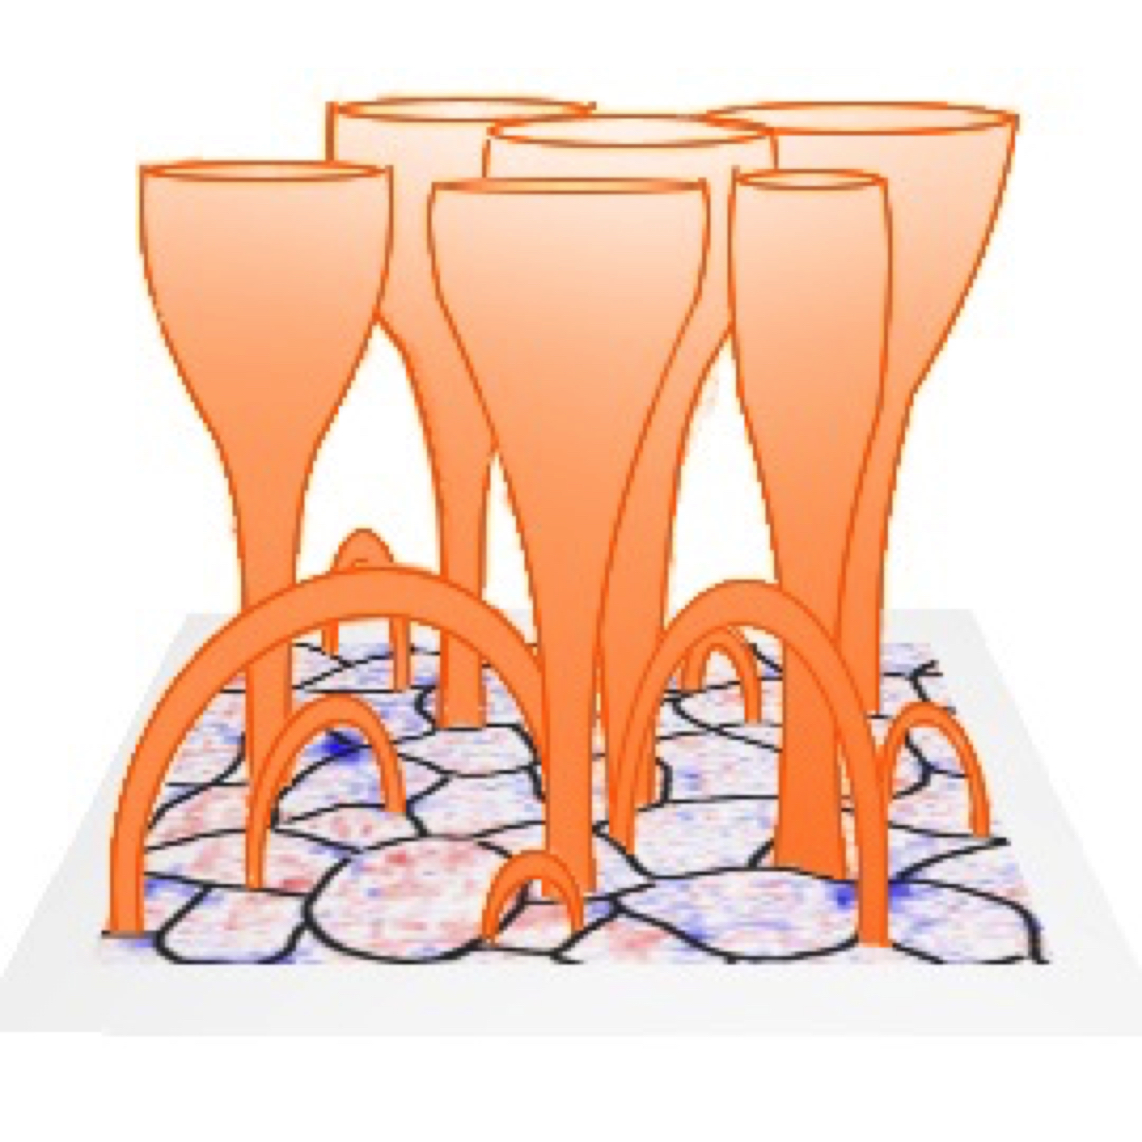
\includegraphics[width=8.5cm]{solar-network-v1.jpg}
\caption{\hl{A schematic} %MDPI: Figures should be placed after their first mention in the paper. Therefore, we have changed the placement for some of the Figures in the manuscript. Please confirm (across the section titles, espessially the first-level sections). MKG confirmed
 representation of the solar magnetic network. 
 \hl{See text for details.} %MDPI: Otherwise, needs to be described. 
%The picture shows the coronal funnels arising from grain boundaries, it also illustrates a range of network loops with temperatures which can be in the range $10^{5}$K to $10^{6}$K. As well as these massive concentrations, the solar magnetogram at the base of the model reveals many north poles in the quiet photosphere, known as the magnetic carpet.  
\label{fig1}}
%\caption{Initial Magnetic Field Configuration, radial field distribution, uniform in the vertical direction with a maximum value of 100G }
\end{figure}
\unskip

\begin{figure}[H]
%\centering
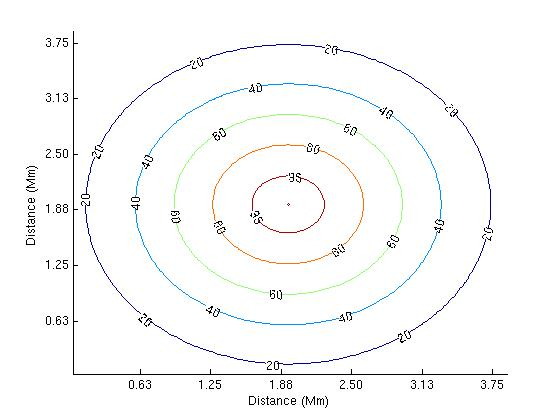
\includegraphics[width=10.5cm]{bfield100G.jpg}
\caption{\hl{The} %MDPI: 1. Please cite the figure in the text and ensure the first citation of each figure appears in numerical order.
                    %2. Please increase the labels and the values of the axes. Invisible otherwise
                    %MKG label sizes increased.
 initial magnetic field configuration showing the radial field distribution {%\bf 
\hl{that}%MDPI: The bold is removed, looks unnecessary.  The following highlights are the same.
} is cylindrical and uniform in the vertical direction with a maximum value of~100 G. The color bar shows the magnetic field strength in Gauss.\label{fig2}}%MKG addedreference to colorbar
\end{figure}

\section{Computational~Model}
The hydrodynamic studies reported in~\hl{Ref.} 
\cite{Griffiths2018b} employed simulation drivers with physical characteristics representing $p$-mode oscillations with varying modes and periods. The~MHD simulations reported here use the same driver and model of the solar atmosphere as used in our initial hydrodynamic study. The~model is  advanced by the inclusion of a uniform, vertical and cylindrically symmetric magnetic~field. 

 The dimensions of the simulation box are $L_{ x}= 4$ Mm,  $L_{y} =4$ Mm and a height of $L_{z} =6$ Mm in the gravitationally stratified $z$-direction. The~computational box is an array of elements 
\highlighting{$128 \times128 \times128 $.} %MDPI: any units? MKG dimensionless number so no units  
The~upper boundary of the model is in the solar corona whilst the lower boundary is coincident with the photosphere. The~MHD code used here is suited to studying the propagation of wave energy from the photosphere, across the transition layer and leaking into the solar~corona. 
 
 %UPDATE
%INCLUDE DETAILS ABOUT THE BOUNDARY CONDITIONS AND THEIR EFFECTIVENESS
The time scales relevant to our study are determined by the 5-minute $p$-mode oscillations; our approach employs boundary conditions allowing us to model induced wave propagation. To~generate these oscillations we use vertical velocity drivers  that are extended across the base of the computational domain. The~mechanism for handling the boundaries is crucial for maintaining the stability of a simulation over many cycles of the 
\highlighting{$p$}-mode 
oscillation. The~challenge is to reduce the reflectivity at the boundaries, in~particular, the~upper and lower boundaries. The~method utilised in these simulations attempts to minimise the gradients near the boundary. Since a central difference method is used to compute the gradients, variable values are copied from the mesh edge into two layers of ghost cells. These layers ensure that the discretization method can be applied over the whole mesh. The~net result of this approach is that any generated perturbation will be effectively propagated out of the computational domain. This type of boundary condition is referred to as an open boundary condition. In~what follows, we describe the model solar atmosphere and the driver employed.
 %UPDATE

Data obtained from solar observations were used to construct a semi-empirical model solar atmosphere, the~resulting model is a representation of the 
 %Quiet 
\hl{quiet} 
Sun. Employing the fundamental assumption of hydrostatic equilibrium, the~VALIIIc model~\cite{Vernazza1981} was used to construct a model of 
the chromosphere in equilibrium. For~atmospheric heights greater than 2.5 Mm, the results from a model of solar coronal heating were used~\cite{McWhirter1975}. The~atmospheric profiles for temperature, density, sound speed and frequency cut-off for this model are shown in Figures~\ref{fig3} and~\ref{fig4}.

\begin{figure}[H]
%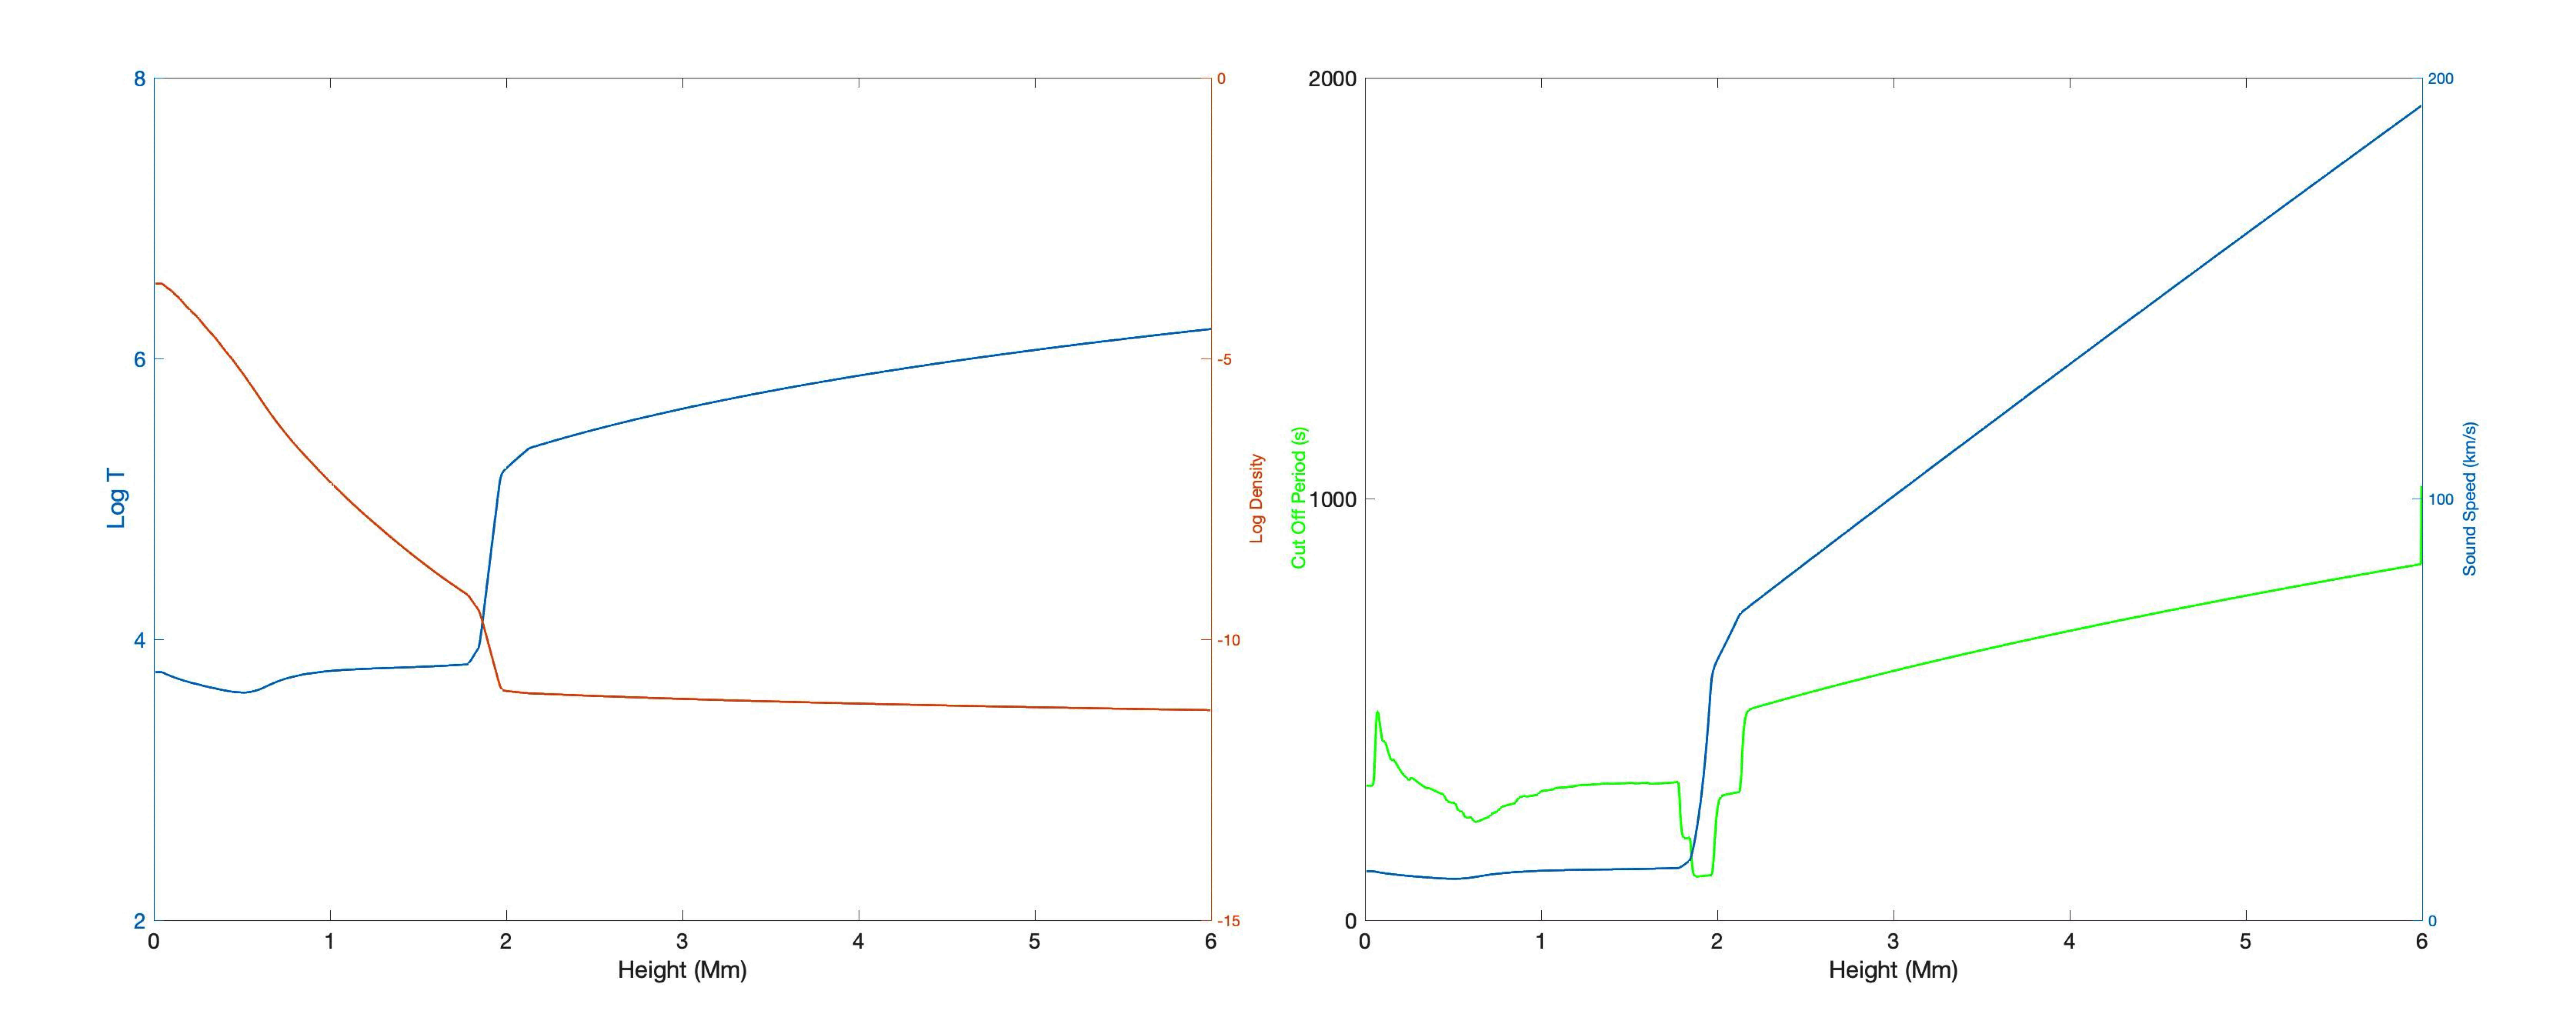
\includegraphics[scale=0.035]{solatmosprofiles.jpg}
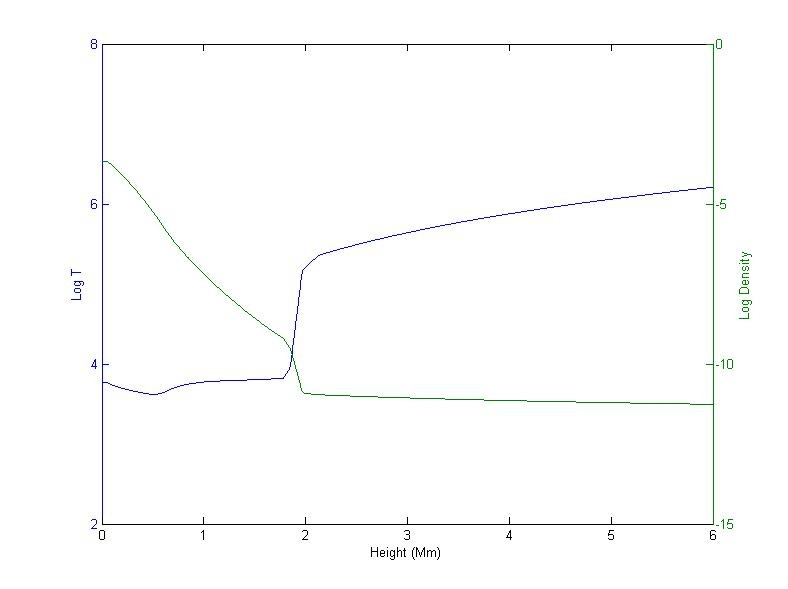
\includegraphics[width=10.5cm]{VAL3C_rho_temp_fig1L.jpg}
\caption{\hl{Atmospheric} %MDPI: Please change the hyphen (-) into a minus sign ($-$, "U+2212"). e.g., "-1" should be "$-$1".
 profiles for the density and temperature for the model solar atmosphere based on the VALIIIc~model~\highlighting{\cite{Vernazza1981}.} %MDPI: helps te hreader.
\label{fig3}}
\end{figure}
\unskip

\begin{figure}[H]
%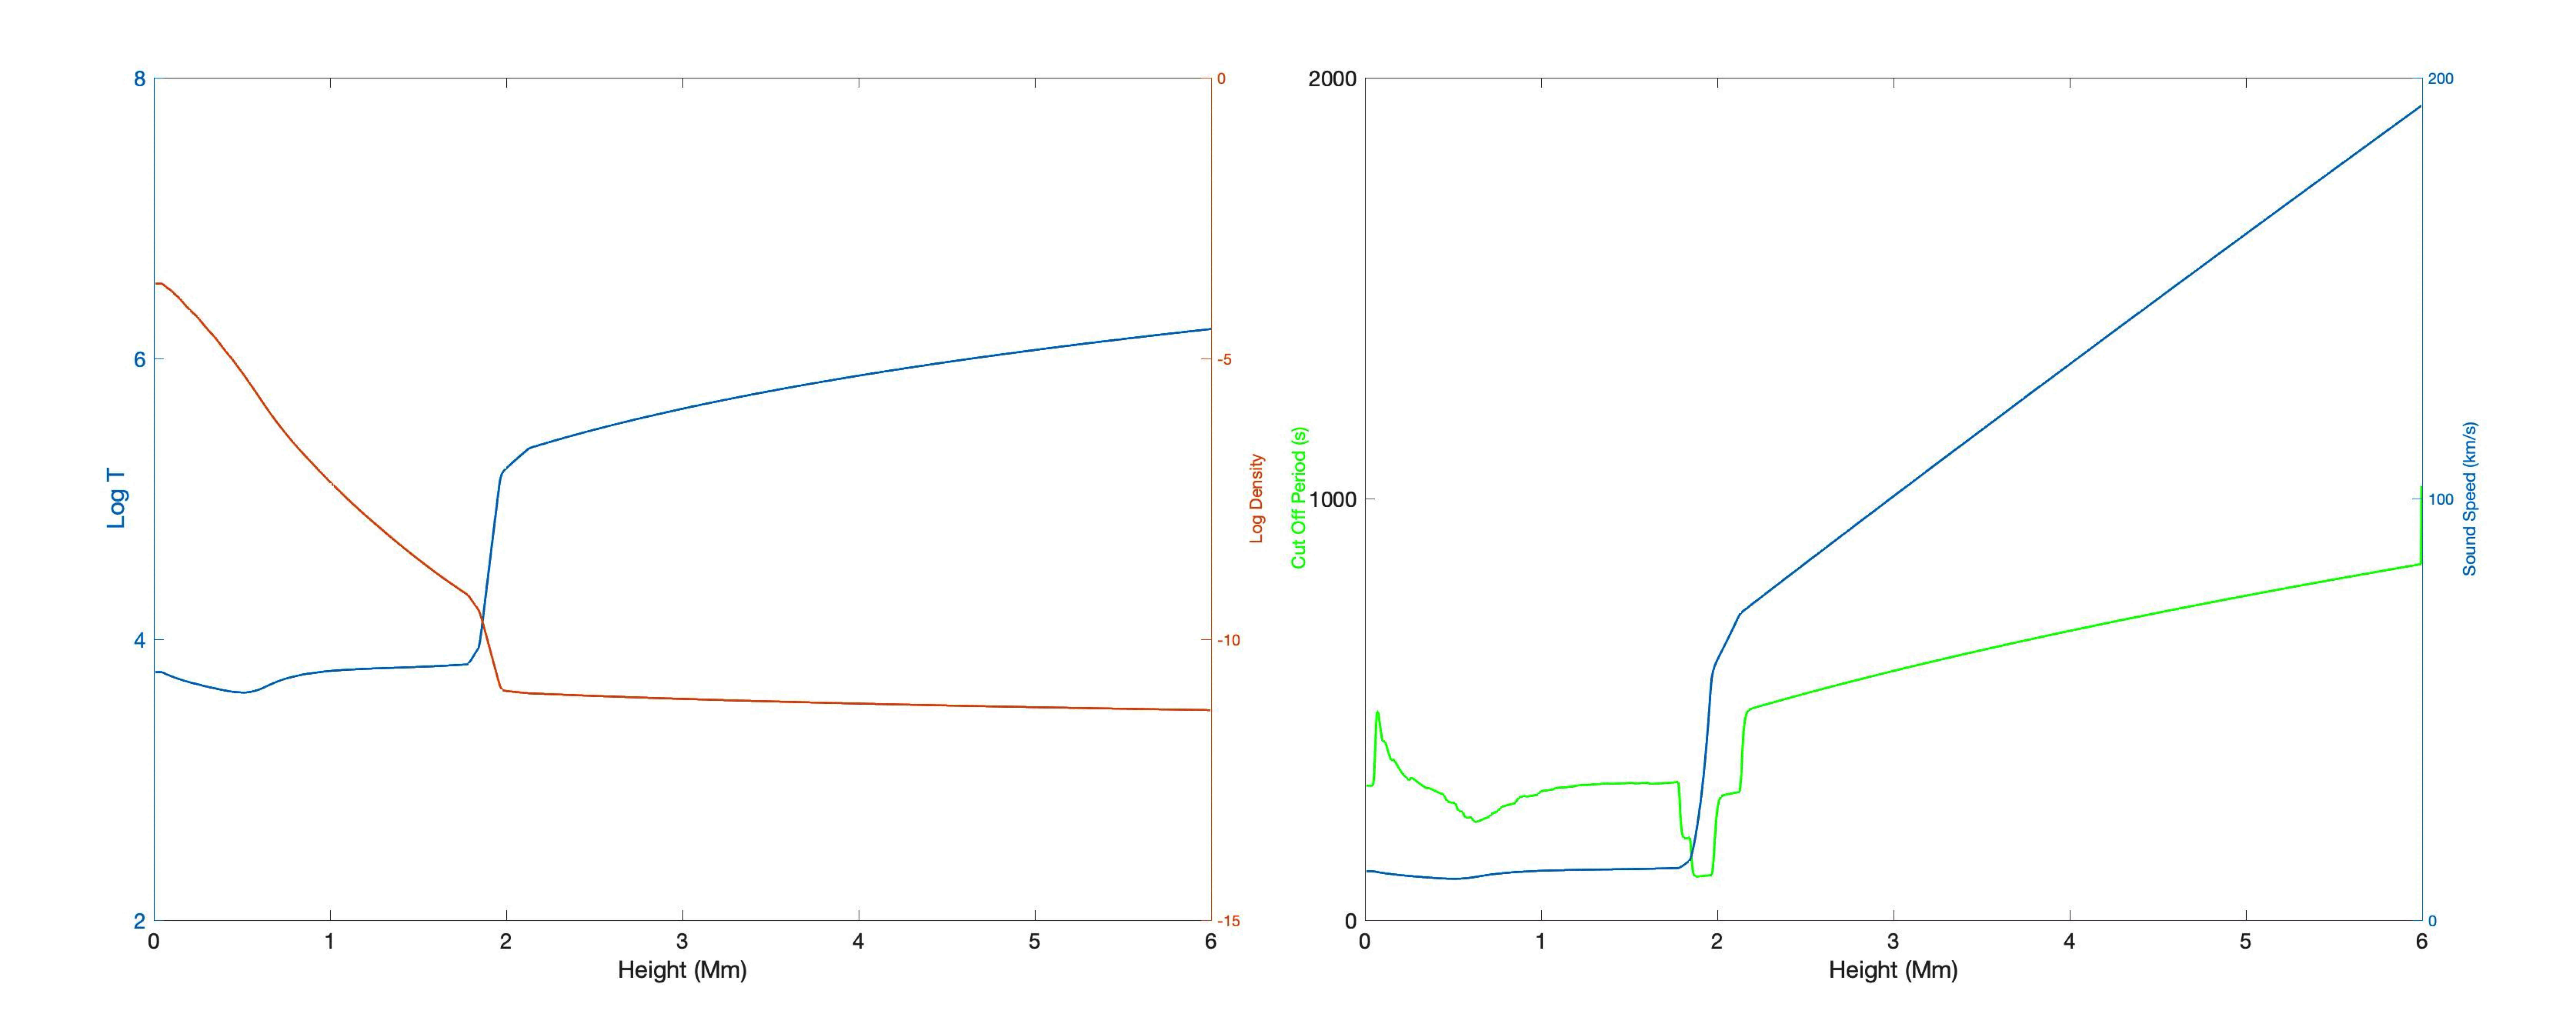
\includegraphics[scale=0.035]{solatmosprofiles.jpg}
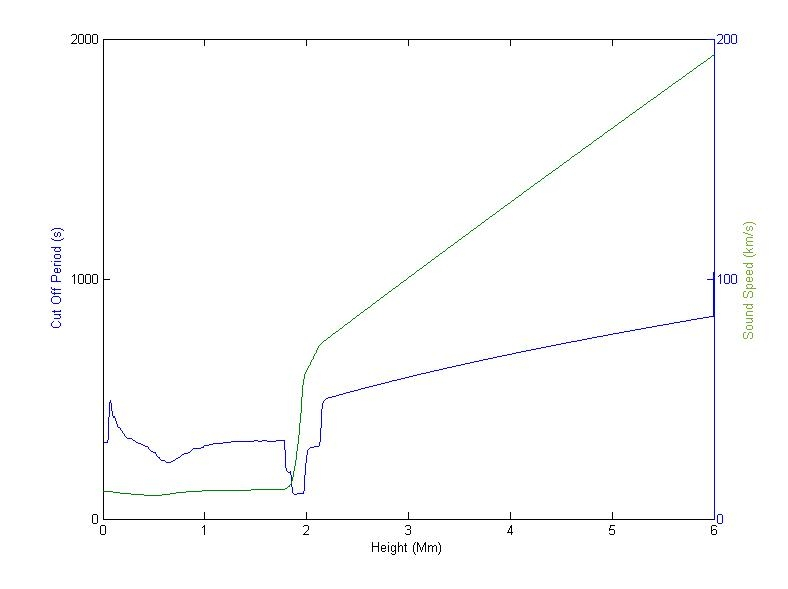
\includegraphics[width=10.5cm]{soundspeedVAL3C_profile_fig1R.jpg}
\caption{Profiles of the computed speed of sound and the frequency cut-off for a solar model atmosphere based on the 
VALIIIc~model~\highlighting{\cite{Vernazza1981}}.
\label{fig4}}
\end{figure}

%\ref{soundspeedVAL3C_profile_fig1R}. 
A further possibility for a model solar atmosphere is the use of the parametric approach; the~smoothed step function used %by
\hl{in Ref.}~\cite{Murawski2010} is an example. Discussion of the validity of model solar atmospheres and realistic models of the chromosphere  indicate the need for observationally derived semi-empirical models, see~\cite{Carlsson1995,Kalkofen2012}. It has been suggested that local dynamo action and joule heating in the dynamical solar chromosphere make the construction of models particularly challenging~\cite{Leenaarts2011}. The~latter aspects are not addressed further in the present~study.


Instead, for~the simulations described here, we use a simplistic model  that is uniform in the vertical ($z$) direction. The~cylindrically 
symmetric field was constructed using  the parametrisation in Equation~(\ref{e7}), the~effective cylinder radius was fixed at $R=0.14$ Mm. 
Simulations were run for different values of \highlighting{$B_{\rm max}$,} %. 
%MDPI: "max", "int", "wave" moved to the normal font as are the words abbreviations, not a variable, formula, indexes. 
\begin{equation}
B_{z}=B_{\rm max} %e %MDPI: the linera case makes it clearer. Please consider. 
\exp{\left(-\frac{x^2+y^2}{R^2}\right)}. 
\label{e7}
\end{equation}

%WHY A CYLINDRICAL FIELD?
A field configuration with vertical cylindrical symmetry is selected as this provides a working, e.g.,~rotational symmetry, representation for  the weaker intra-network magnetic field. The~choice of working geometry is a convenience when coding the MHD~equations.

%RE: if we have 50 G, that is far too weak for a pore. i siggest to delete this:
%a solar pore.    A good discussion of the structure of  solar pores can be found in \citet{Simon1970}, \citet{Cameron2007}.
Since the field is uniform in the vertical direction, the model atmosphere is in magnetohydrostatic equilibrium. This was checked by ensuring that the initial configuration satisfies the magnetohydrostatic balance, for~an example see~\cite{Schussler2005,Gent2013}. We also explicitly tested that the there were no dynamic changes in the model due to a magnetohydrostatic imbalance. The~resulting density and temperature profiles are shown in Figure~\ref{fig3}. 


\section{Numerical Drivers for $p$-Mode~Oscillations}



The simulations, presented in this paper, employ an extended driver resulting in the perturbation of the entire lower boundary of the model.  The~photospheric $p$-mode oscillations  that are observed on the Sun have a horizontal wavelength and coherence. The~vertical velocity driver used here is an acoustic $p$-mode driver located at the photosphere and exciting waves which propagate into our realistic 3D model geometry of the solar atmosphere. An~extended driver with a sinusoidal dependence and a wavelength of 8~Mm applied along the middle of the base of a computational domain of dimension 4 Mm represents  a 
\highlighting{{\it fundamental mode}} %MDPI: is italics necessary? Reserved for subtitles.   
component of the global acoustic oscillations. Drivers may be constructed as an ensemble of these solar global eigenmodes. The~driver is approximated by the 
 \hl{expression,} %MDPI: clear enough. Please consider.  
 % shown in Equation~(\ref{e8}): 


%%\begin{tabular}{ccc}
\begin{equation}
 V_{z}  =  A_{nm} \sin\left(\frac{2\pi t}{T_s} \right)\sin\left(  \frac{(n+1)\pi x}{L_x} \right)  
 \sin\left(\frac{(m+1)\pi y}{L_y} \right) \exp\left( -\frac{(z-z_0)^2}{\Delta z^2} \right). %,
\label{e8}
\end{equation}
%%\end{tabular}

For the  simulations here, a~$p$-mode driver corresponding to the 5-minute mode was used with period 300 s and mode (2,2) as an example. Earlier studies demonstrated the effectiveness of this mode with energy propagation, see~\cite{Griffiths2018b}. Simulations were run for different values of the magnitude of the magnetic field. The~mode numbers identified here are the $n$ and $m$ values in the expression for the driver shown in Equation~(\ref{e8}).

%FIXME
%DRIVER LOCATED IN THE PHOTOSPHERE WHY AT THE TEMPERATURE MINIMUM WHY NOT BELOW IDEALIZED EVANESCENCE NATURE OF SURFACE IS DYNAMIC










For the driver equation given in Equation~(\ref{e8}), $T_{s}$ is the period, $A_{nm}$ is the amplitude, the~indices $n$ and $m$ define the mode and the~lengths of the base of the simulation box in the $x$ and $y$ directions are $L_{x}$ and $L_{y}$, respectively. The~driver width, $\Delta z$ is set to $4$~km, the~parameter $z_{0}$ was set so that the vertical location of the driver is in the photosphere, 0.5 Mm above the lower boundary of the model and coincident with the location of the temperature minimum. The~simulations presented employ the parameter $A_{nm}$ = 500\, ms$^{-1}$ with the mode indices set to $n,m=2$. 


\section{Global Magnetoacoustic Waves in Uniform Vertical Magnetic Field~Configurations}

Magnetohydrodynamic simulations have been performed with $p$-mode oscillations of the photospheric layer and for magnetic field strengths of 0 G, 50 G, 75 G and 100~G. The plasma-$\beta$ was determined for the case with a magnetic field strength of 100 G. The~plasma-$\beta$ for the model decreases rapidly from a value of 50 at 0.7 Mm above the lower boundary of the simulation domain; $\beta$ is 1 at a height of 1.39 Mm.  
%It is anticipated that for the region with $\beta \approx 1$, mode conversion may occur. 

%FIXME
%REFEREE COMMENT BELOW ADDRESS THIS

%%Vertically propagating acoustic waves in the vertical magnetic field cannot have mode conversion.

 %% Figure~3  \ref{vzplot_bv100g_76_150_225}
 Figure~\ref{fig5} %%\ref{vzplot_bv100g_76_150_225} 
 shows the vertical component of the velocity at various times for different sections through the simulation box. Each plot in  Figure~\ref{fig5} %% \ref{vzplot_bv100g_76_150_225}
 corresponds to a vertical field configuration with a maximum field strength of 100~G. Figure~\ref{fig6} provides a comparison with the 0~G case and %%\ref{vzplot_bv0g_76_150_225}
 illustrates a clear difference between the purely hydrodynamic and the MHD case. The~figures for the MHD case exhibit evidence of a fast moving magnetoacoustic wave mode. The~measured propagation speed is consistent with that of a fast magnetoacoustic mode. Figures~\ref{fig5} and \ref{fig6} compare the wave modes at one-quarter, half and three-quarters of a~cycle. 
 
 \begin{figure}[H]

\begin{adjustwidth}{-\extralength}{0cm}
\centering %% If there is a figure in wide page, please release command \centering
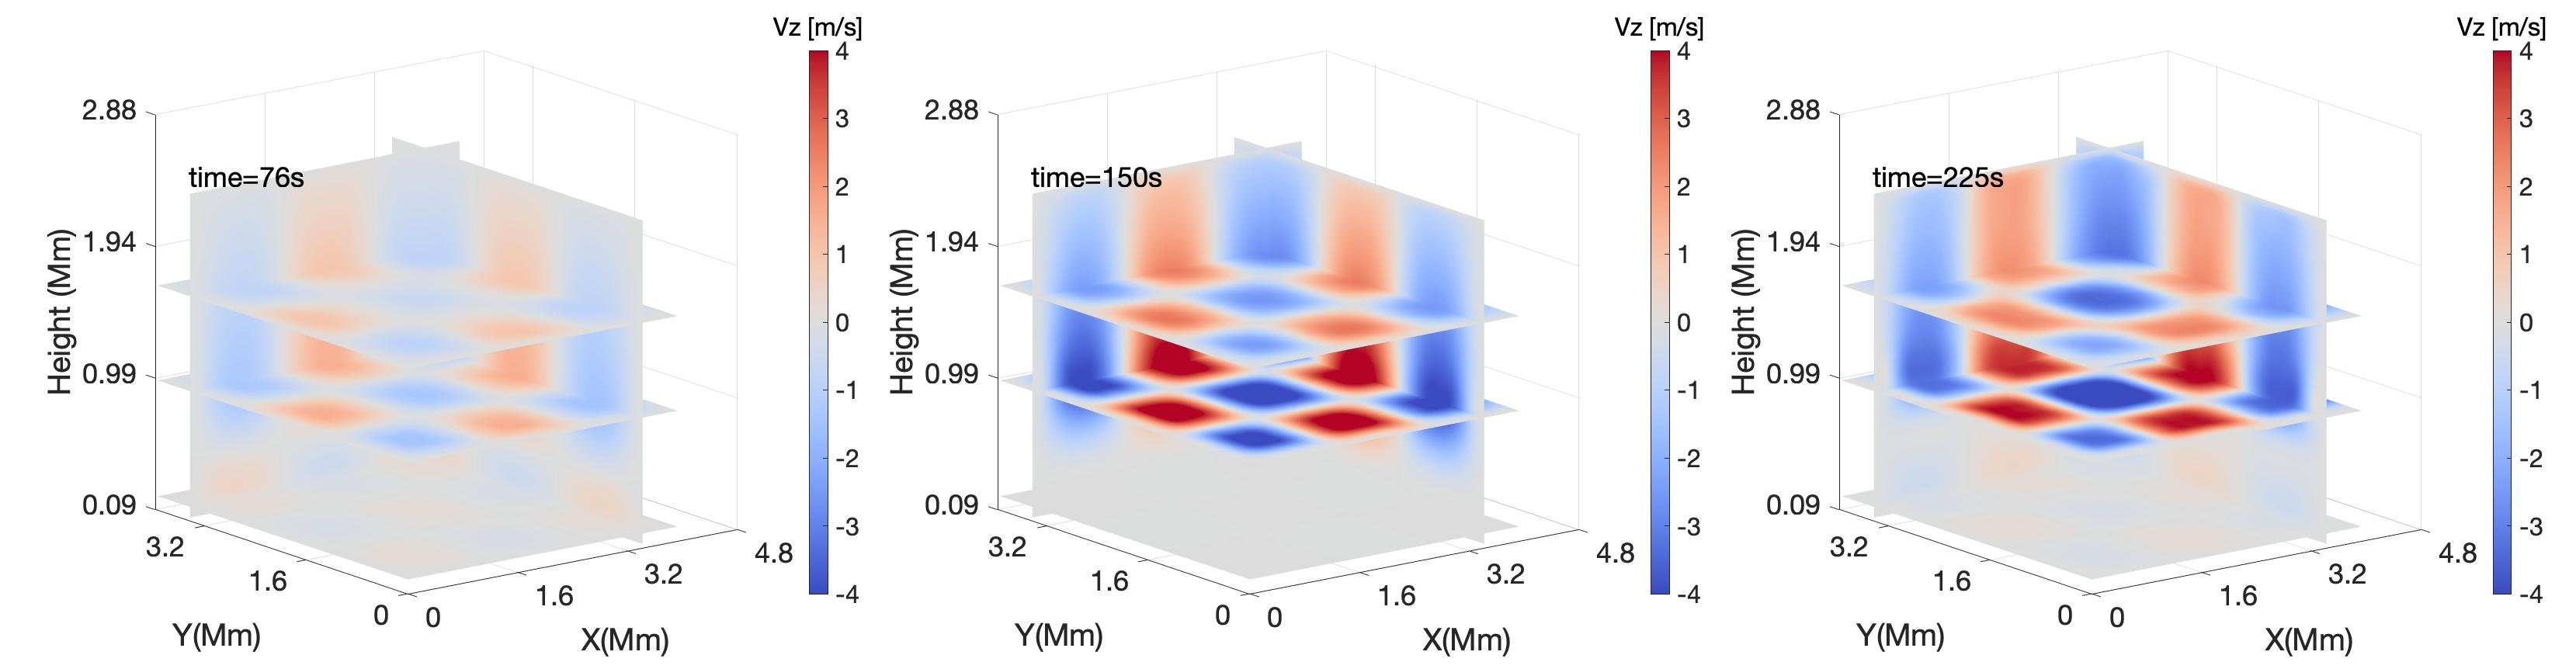
\includegraphics[scale=0.05%5
]{vzplot_bv100g_76_150_225.jpg}
\end{adjustwidth}
\caption{\hl{The vertical} %MDPI: 1. Please change the hyphen (-) into a minus sign ($-$, "U+2212"). e.g., "-1" should be "$-$1".
                      %2. Figure size increased for better visibility. please confirm. 
                      %MKG confirmed
component of the velocity for different sections of the simulation after different times 76 s, 150 s and 225 s for a vertical field with maximum field of~100 G.\label{fig5}}
\end{figure}


\begin{figure}[H]
\begin{adjustwidth}{-\extralength}{0cm}
\centering %% If there is a figure in wide page, please release command \centering
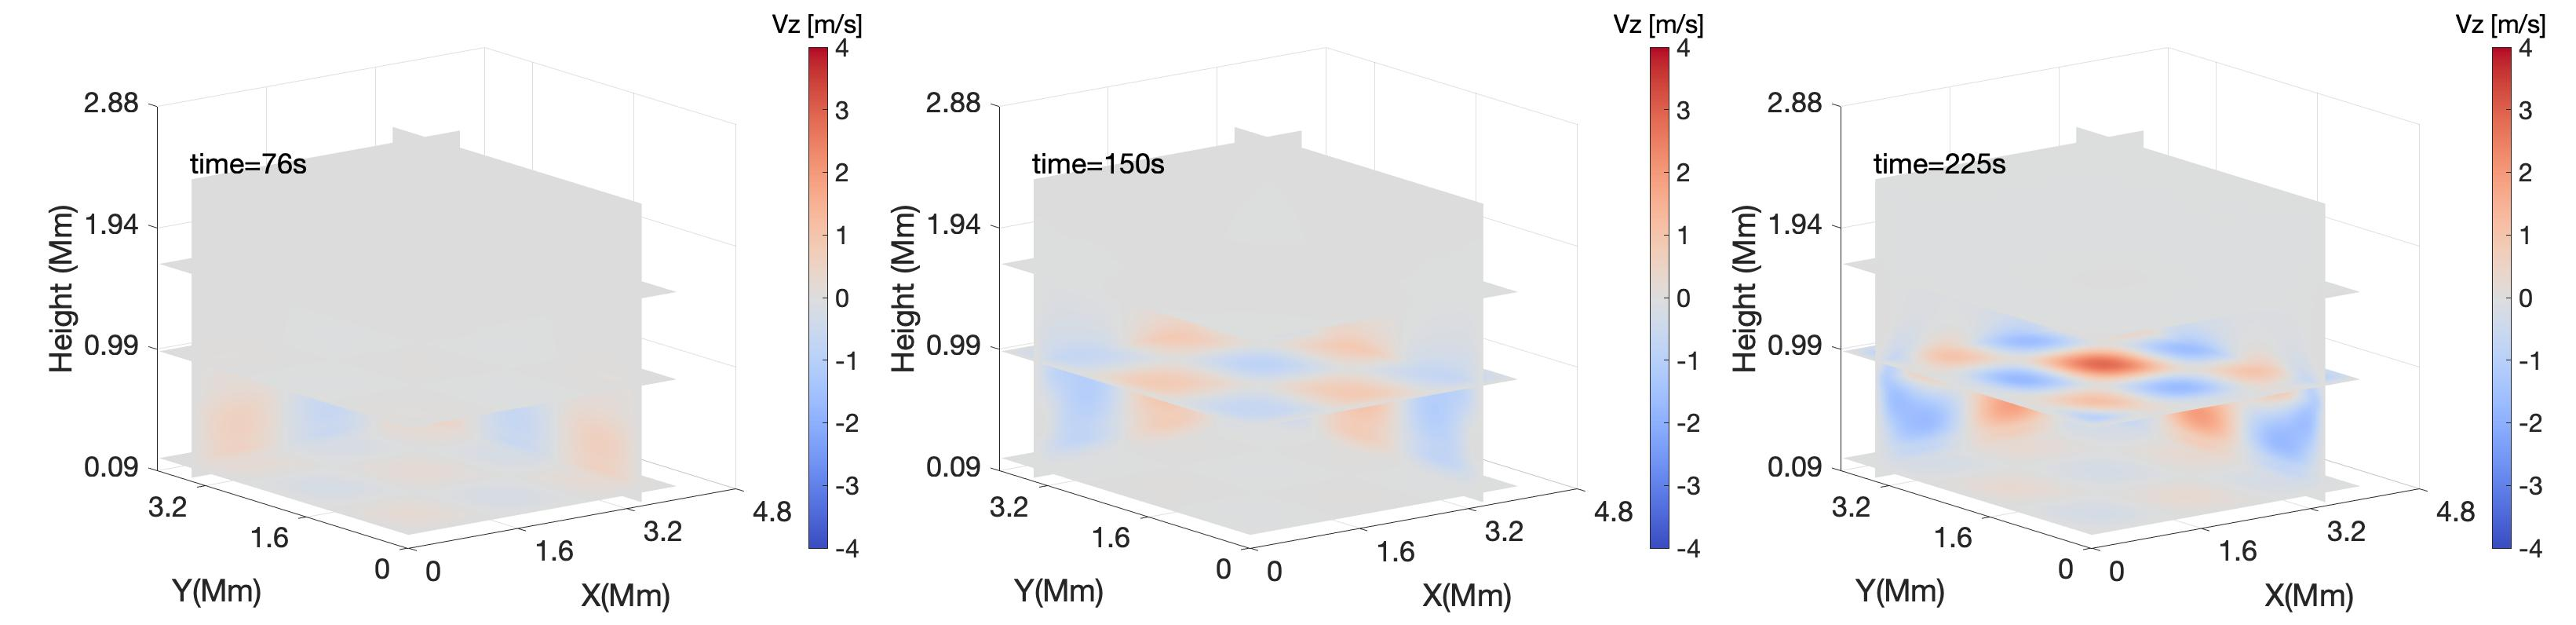
\includegraphics[scale=0.05%5
]{vzplot_bv0g_76_150_225.jpg}
\end{adjustwidth}
\caption{\hl{The vertical} %MDPI: 1. Please change the hyphen (-) into a minus sign ($-$, "U+2212"). e.g., "-1" should be "$-$1".
                            %2. Figure size increased for better visibility. please confirm.
                            %MKG Confirmed
 component of the velocity for different sections of the simulation after different times 76 s, 150 s and 225 s for a magnetic field of~0 G.\label{fig6}}
\end{figure}


A set of videos of all the simulations that were performed can be obtained from the online research data archive hosted by The University of 
Sheffield %, \citet{Griffiths2018a} 
\highlighting{\cite{Griffiths2018a}} %MDPI: or "by Griffiths, ... " adding all three authors. 
 %{\bf RE: pls provide a direct weblink here. MKG the refernce is a working direct link}. 
 The videos display the evolution of the $z$-component of the plasma velocity along different layers of our model solar atmosphere. Each video shows the value of the vertical component of the plasma velocity ($z$-component in m/s) along different slices through the simulation box. Each video is labelled using the magnetic field strength in Gauss. Inspection of these results reveals that there are channels along which the vertical component of the plasma velocity is enhanced, and these are concentrated towards the central region of the simulation~box.
  %Figure 6 shows the normalised difference between the results for the 100G case and the 0G case. The normalisation is achieved by dividing the difference value  by the sum the sum of the values for the 0G and 100G case. The largest difference arises at the height where the velocity reverses direction.   



 
  
  %Our
 \hl{The} 
 results \hl{obtained} 
indicate that even a small magnetic field appears to enhance the motion of plasma in the low corona and  there is an apparent difference in phase between the magnetic field cases. As~well as an increase in the velocity amplitude with increasing magnetic field there is a small variation in the frequency of the oscillation. In~order to address  the observed variation in frequency, further investigative simulations would be required  that would include simulations running for a larger number of cycles.  The~key point here is that the background magnetic field is vertical, one may not accept any frequency variation assuming a linear wave evolution is the key component to the physics. Since the simulations do show small frequency variations, this may mean that that the linear theory may break.
  %For magnetic fields with strengths between $1$ kG and $50$ G, the theoretical prediction of \citet{Hindman1996} resulted in frequency shifts in the microhertz and nanohertz range.  Although this was a prediction of helioseismology, their result still provides insight into the mechanism of frequency shifts of waves in atmospheric magnetic structures. 
  




%\begin{figure*}\label{vzplot_bv100g_0g_76_150_225}
%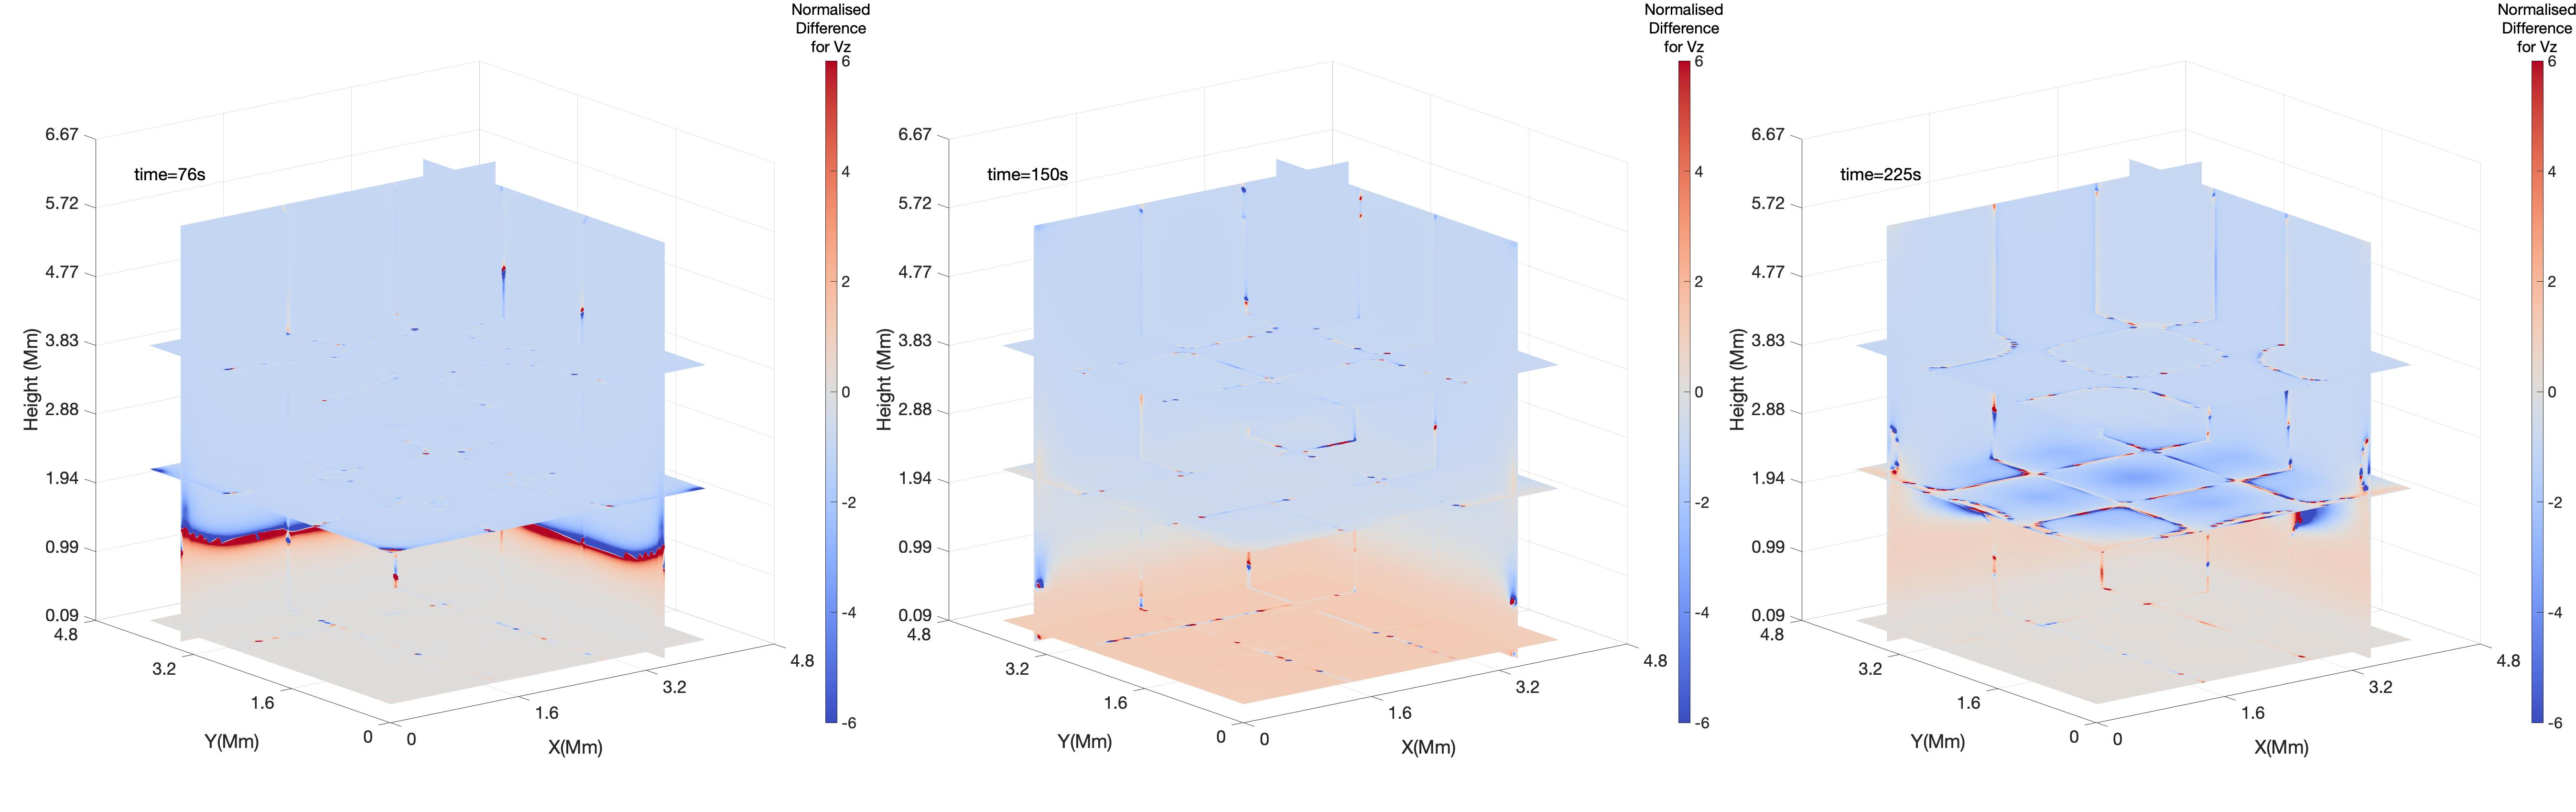
\includegraphics[scale=0.023]{vzplot_dif_bv100g_0g_76_150_225.jpg}
%\caption{The Normalised Difference of the Vertical Component of the Velocity for Different Sections of the Simulation for 76s, 150s and 225s for a magnetic field of 100G.}
%\end{figure*}
%FIXME
%MENTION HERE WHY WE HAVE CUT THIS OFF AND REFERE TO BOUNDARY CONDITIONS AND PROBLEMS OF REFLECTION

After much  effort implementing and testing  the chosen numerical scheme to solve the numerical equations, there are still reflections at the boundary; therefore, we consider the simulations to be valid up to the point where reflection occurs. Because~of this, the~simulations are cut after approximately 600~s of real time, corresponding to two period~cycles.

A  time--distance plot for the 300~s period driver, with~the 
 \hl{100~G} %MDPI: looks Figure 8 to come before Figure 7, the latter shows the 0 G case. Please see just below and correct accordingly. 
field is shown in \highlighting{Figure~\ref{fig7}}%MDPI: Figures should be numbered in order of appearance. We detected "Figure 8" appears before "Figure 7", please rearrange all the references to appear in numerical order. MKG numerical references corrected as requested
. The~reflections from the imperfect boundary conditions result in increased velocity amplitudes after a few oscillations. Although~we are investigating the propagation of waves into the corona, the~time--distance plots emphasise phenomena observed in the chromosphere and around the transition zone.  The~wave speeds measured from this time--distance plot are shown in Table~\ref{tab1}. A~comparison with the wave speeds computed from the model atmosphere suggests that the~speeds for the 0 G field are consistent with the speed of sound in the solar atmosphere, whilst the speeds for the non-zero magnetic field are consistent with propagation speeds for magnetosonic modes.
For a  vertical magnetic flux %tube 
with magnetic field strength $B_{0}$ and internal density $\rho_{0}$, comparisons with the measured wave speeds were computed using the following definitions:
the speed of sound,
\begin{equation}
 c_{s}  =    \sqrt{\frac{\gamma p_0}{\rho_0}}, 
\label{e10}
\end{equation}
the Alfv\'en speed,
\begin{equation}
 v_{A}  =    \sqrt{\frac{B_{0}^{2}}{\mu\rho_{0}}},  
\label{e11}
\end{equation}
the magnetoacoustic wave speeds, also known as  the slow or cusp or tube speed,
\begin{equation}
 c_{t}  =    \frac{c_s v_A}{\sqrt(c_s^2+v_A^2)}, 
\label{e12}
\end{equation}
and the kink speed,
\begin{equation}
 c_{k}  =    \sqrt{\frac{\rho_0}{\rho_0+\rho_e}}v_A.
\label{e12}
\end{equation}

\begin{figure}[H]
%\centering
%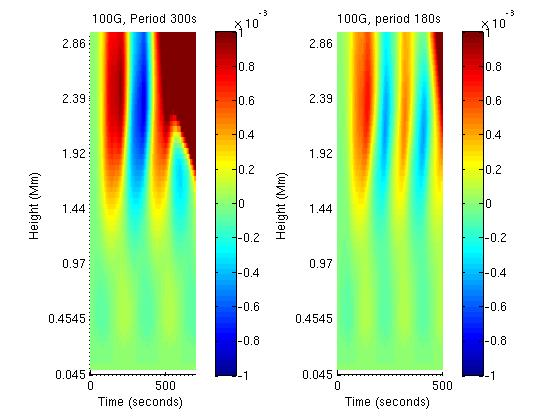
\includegraphics[scale=0.475]{dt_vvert_100G_300s_180s.jpg}
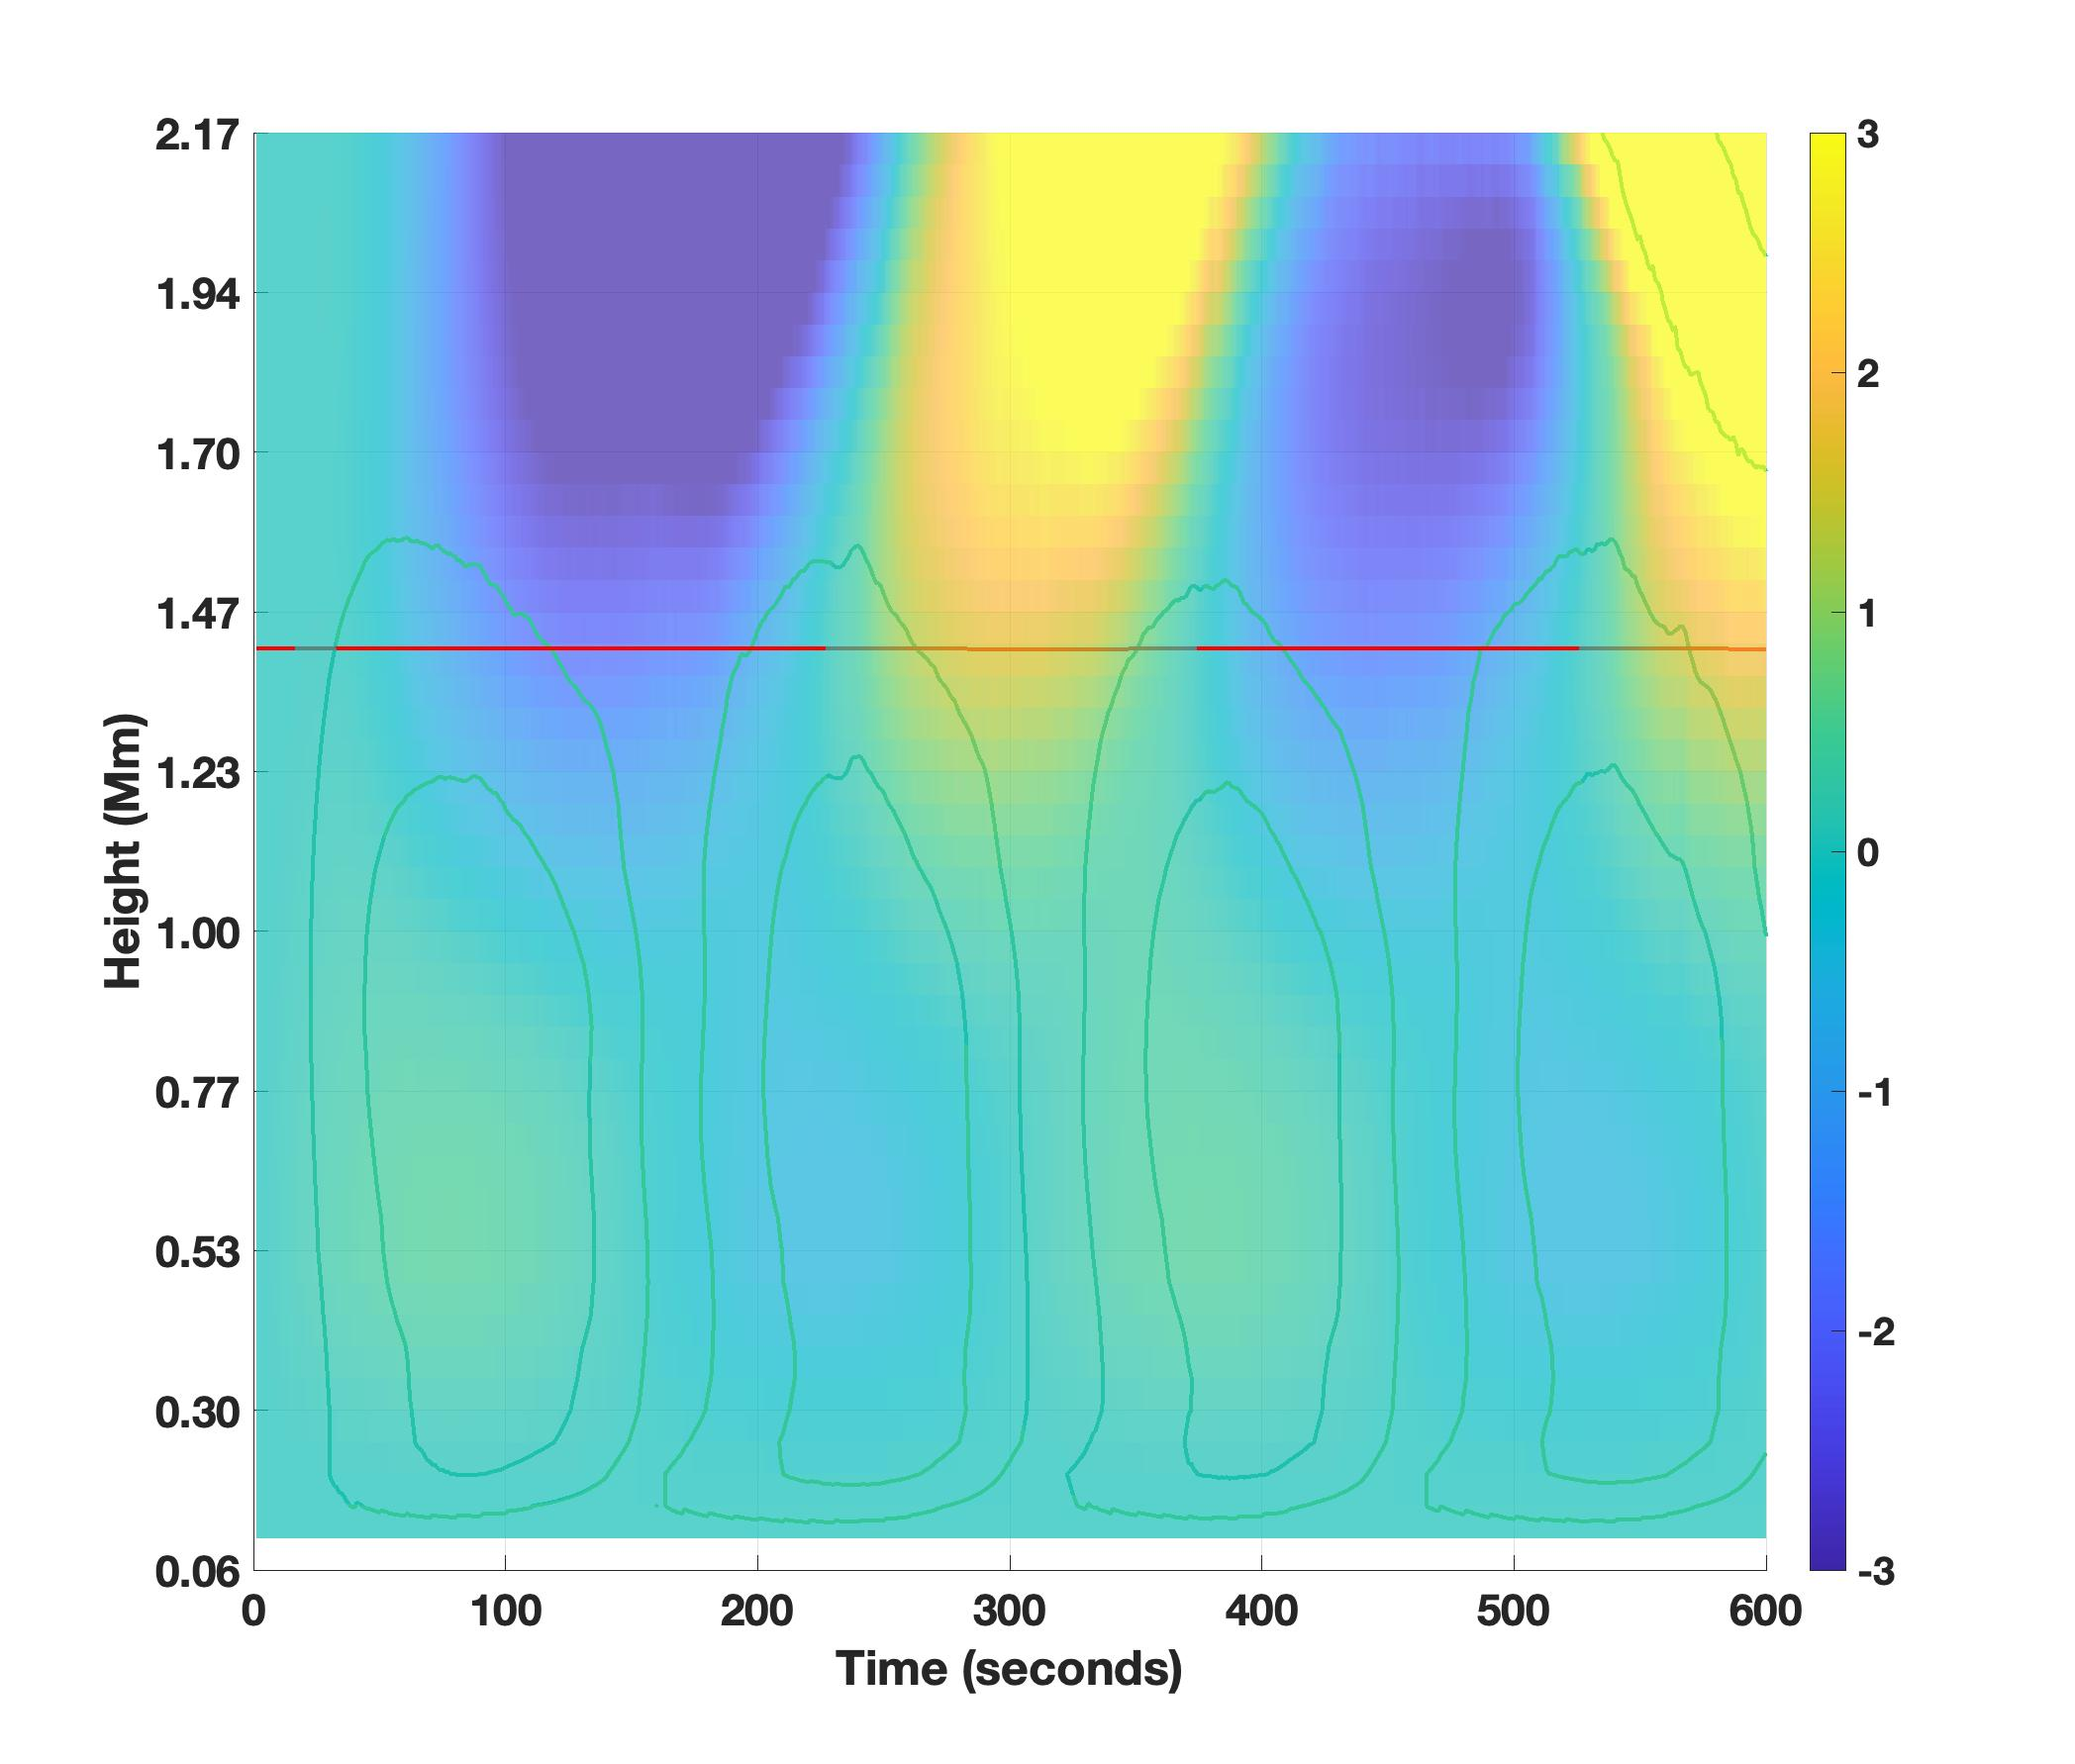
\includegraphics[width=10.5cm]{td_vert_bv100G_300_with_bandbeta.jpg}
\caption{\hl{Time--distance} %MDPI: 1. Please change the hyphen (-) into a minus sign ($-$, "U+2212"). e.g., "-1" should be "$-$1".
                             % 2. Please increaase the size of the axes labels and the values on the axes. Invisible otherwise. %MKG axis label sizes increased
 plot of the vertical component of the velocity in the mid-chromosphere, for~the magnetic field of 100~\hl{G. %, the
The~central} %MDPI: fits better a new sentence.
red line is the line for plasma-$\beta$  equal to~1.\label{fig7}}
%\caption{Energy Flux for the mid-section of the Simulation for 76s, 150s, 225s and 330s for a vertical field with maximum field of 50G }
\end{figure}


\begin{table}[H]%\label{wavespeeds}
\caption{\hl{The %table shows wave %MDPI: 1. clear enough. 2. No secondary \midrule necessary.
speeds} obtained from the  time--distance plots for the 300~s period driver with magnetic fields of 0~G, 50~G, 75~G and 100~G.\label{tab1}}
%\label{Tablewavespeeds_300s}
%\centering
\newcolumntype{C}{>{\centering\arraybackslash}X}
\begin{tabularx}{\textwidth}{c C C C C}
\toprule
\textbf{Wave Speed (km/s)}   &  \textbf{0 G}  &  \textbf{50 G} &  \textbf{75 G} & \textbf{100 G}\\
 \midrule
2 Mm & 12.6  &   96.5       &   47.7      &  25.2     \\
 %\midrule
1 Mm & 10.1  &    64.1      &   44.4     &   45.4      \\
 %\midrule
0.5 Mm & 8.7  &   45.4      &   37.8      &   32.3    \\
\bottomrule

\end{tabularx} 

\end{table}
\unskip

The results indicate a variety of waves. Inspection of Figure~\ref{fig8} reveals excitation from the driver along with quasi-standing oscillations in the chromospheric cavity. There is also partial reflection of the signal at the boundary of the chromosphere and the transition layer. The~results also display evidence for signals propagating horizontally at the transition region and with frequencies similar to that of the driver. The~time--distance plot in Figure~\ref{fig7}, for~the 100~G case, exhibits reduced reflection at the transition layer, indicating energy leakage into the solar corona. Figure~\ref{fig7} shows an initial fast mode pulse followed by slow mode oscillations above the line which correspond to a plasma-$\beta$ with a value of one. Below~the height of 1~Mm, we observe quasi-standing mode oscillations along with oscillations of the magnetic field perturbations. Below~0.3~Mm, the~driver oscillations can be observed in conjunction with possible magnetoacoustic slow mode oscillations. Since the source terms perturb only the vertical component of the velocity and the model is cylindrically symmetric, pure Alfv\'en modes are not~expected.




%FOR THE FOLLOWING FIGURE THE NORMALISATION USED DEVELOPS UNPHYSICALLY LARGE COULD PROJECT V FIELD ONTO WAVE PROPAGATION DIRECTION


\begin{figure}[H]
%\centering
%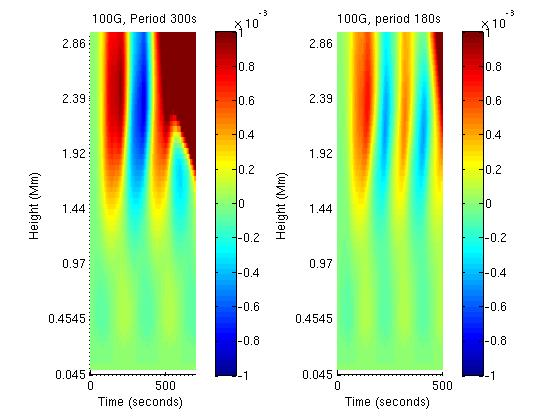
\includegraphics[scale=0.475]{dt_vvert_100G_300s_180s.jpg}
%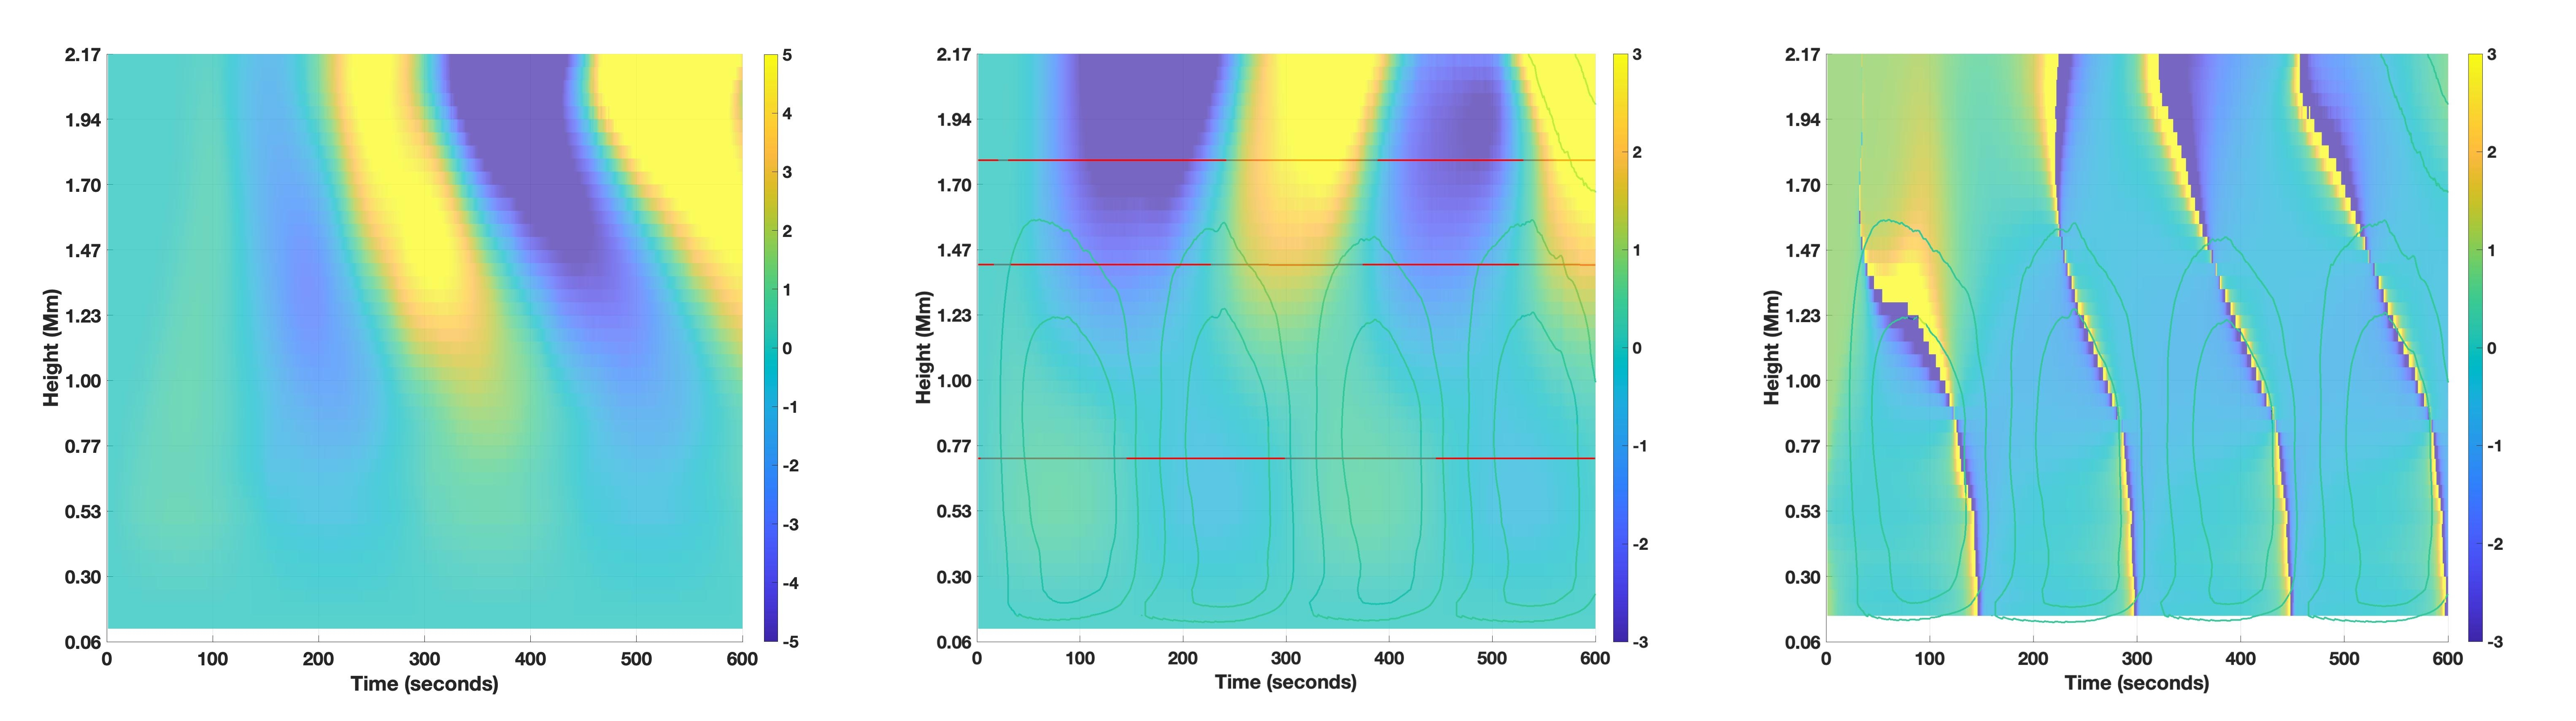
\includegraphics[scale=0.02]{dt-0G-100G-dif-plot.jpg}
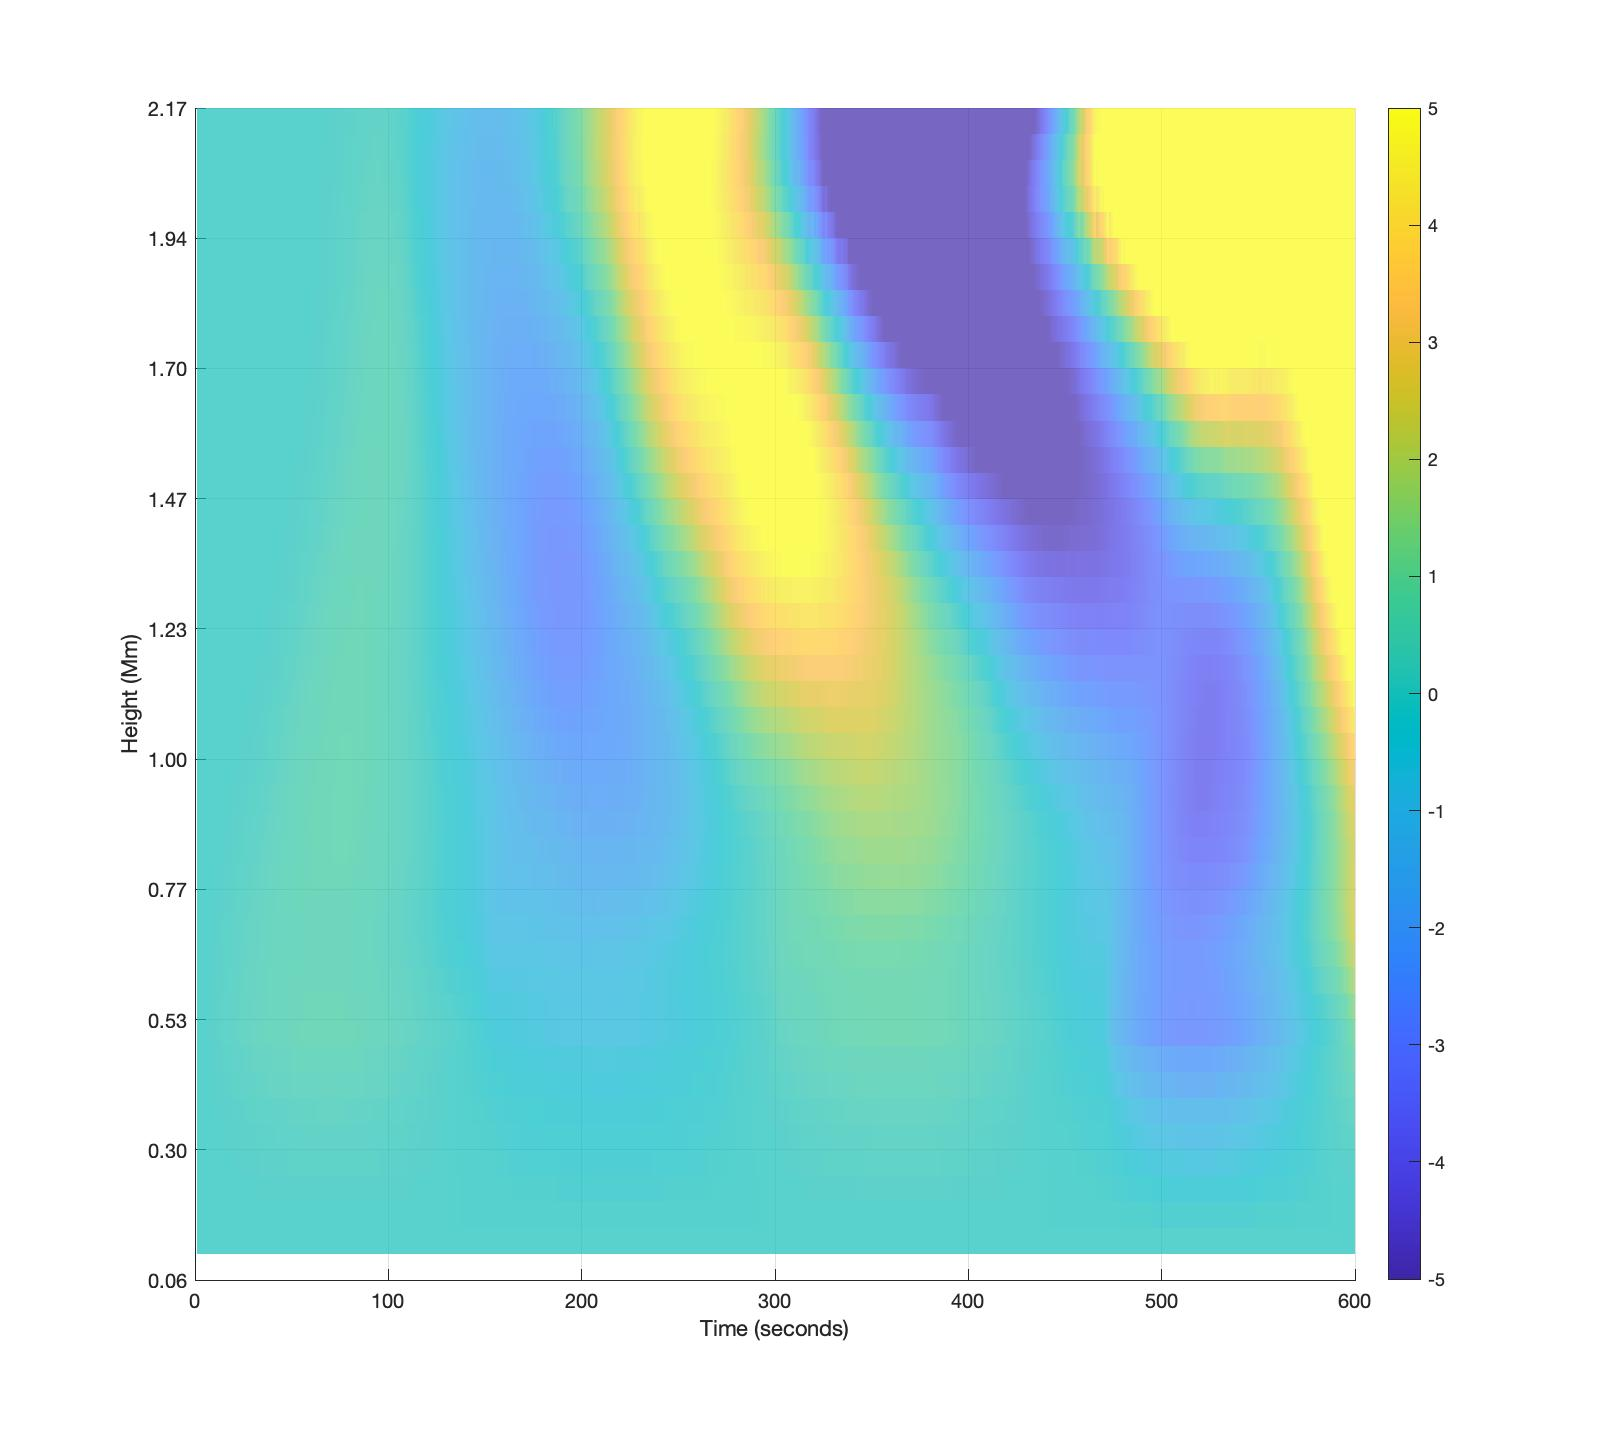
\includegraphics[width=10.5cm]{td_vert_bv0G_300.jpg}
\caption{\hl{Time--distance} %MDPI: 1. Please change the hyphen (-) into a minus sign ($-$, "U+2212"). e.g., "-1" should be "$-$1".
                 %2. Please increaase the size of the axes labels and the values on the axes. Almost invisible otherwise. %MKG axis label size increased
 plot of the vertical component of the velocity in the mid-chromosphere, for~a magnetic field of 0~G.\label{fig8}}
%\caption{Energy Flux for the mid-section of the Simulation for 76s, 150s, 225s and 330s for a vertical field with maximum field of 50G }
\end{figure}
\unskip



The time--distance plots displaying the vertical component of the plasma velocity indicate significant differences in the propagation 
behaviour for the hydrodynamic and non-zero magnetic field cases. It is necessary to understand and quantify the extent of the energy 
leakage into the solar atmosphere. To~investigate the influence of the magnetic field on the propagation of wave energy we employ an 
expression for the energy flux which was used by~\cite{Bogdan2003}. The~wave energy flux 
 \hl{${\bf F}_{\rm wave}$} %MDPI: No bold for "wave" seems necessary, so removed.
 is given by
$$
{\mathbf F}_{\rm wave}=\tilde{p}_{k} {\mathbf v}+\tilde{\mathbf B}\cdot {\mathbf B_{b}}{\mathbf v}+{\mathbf v}\cdot \tilde{\mathbf 
B}{\mathbf B_{b}} .
$$

We compute the \hl{time-averaged} %MDPI: teh dash clarifies. Unclear otherwise. 
energy flux integrated over different cross sections of the simulation \hl{box:} %.
\begin{equation}
F_{\rm int}= \frac{1}{t_{\rm max}} \int_{0}^{t_{\rm max}} \int {\mathbf F}_{\rm wave} \cdot d{\mathbf A}dt,
\label{e11}
\end{equation}

These expressions are dependent on the perturbed kinetic pressure $\tilde{p}_{k}$. The perturbed variables are represented with a tilde  on top of the variable and a subscript $b$ for the background variables. 
%. %MDPI: Please expalin the tilde on top of the variables.
$$
\tilde{p}_{k}=\left(\gamma - 1\right)\left( \tilde{e}-\frac{ \left( \tilde{\rho} +\rho_b \right){\mathbf v}^2}{2}-\frac{{\mathbf B}^2}{2}\right).
$$


Using Equation~(\ref{e11}), we computed the energy flux integral for each of the drivers at different atmospheric heights and averaged over the total time. Next, we compute the ratio of this integrated energy flux to the integrated energy flux at the location of the driver. The~resulting values are shown in Table~\ref{tab2}. It appears that for heights greater than 4~Mm, the~energy flux is enhanced for increasing values for the vertical magnetic field. In~Figure~\ref{fig9},
%\ref{energyfluxratio_50G_75G_100G_line},
we plot the ratio of the integrated energy flux ratio for different values of the field at different heights and for the different vertical field values (the blue, orange, purple and red  are for field values of 0~G, 50~G, 75~G and 100~G, respectively). These plots demonstrate that for higher $B$-field magnitudes there is a small leakage of energy propagation. This latter finding is interesting because this is consistent with observations and other simulation results that demonstrate an enhancement for inclined~fields.

\begin{table}[H]%\label{energyflux}
\caption{\hl{The %table shows the 
time-averaged} and integrated energy flux ratio obtained  for the 300~s period driver with magnetic fields of 0~G, 50~G, 75~G and 
100~G.\label{tab2}}
%\label{energyfluxratio}
%\centering
\newcolumntype{C}{>{\centering\arraybackslash}X}
\begin{tabularx}{\textwidth}{c C C C C}
\toprule
\textbf{Magnetic Field (G)}   &  \textbf{1 Mm}  &  \textbf{2 Mm} &  \textbf{4 Mm} & \textbf{5.5 Mm} \\
\midrule
0 G & 0.155  &    $-$1.771 $\times$ $10^{-5}$      &   1.227 $\times$ $10^{-6}$     &   8.194 $\times$ $10^{-7}$      \\
%\midrule
50 G & 0.270  &   $-$0.399       &   0.040      &  0.021     \\
%\midrule
75 G & $-$0.507  &    $-$0.126      &   0.015     &   0.007      \\
%\midrule
100 G & $-$0.255  &   $-$0.226      &   0.019      &   0.006    \\
\bottomrule

\end{tabularx} 
\end{table}

\begin{figure}[H]
    %\centering
    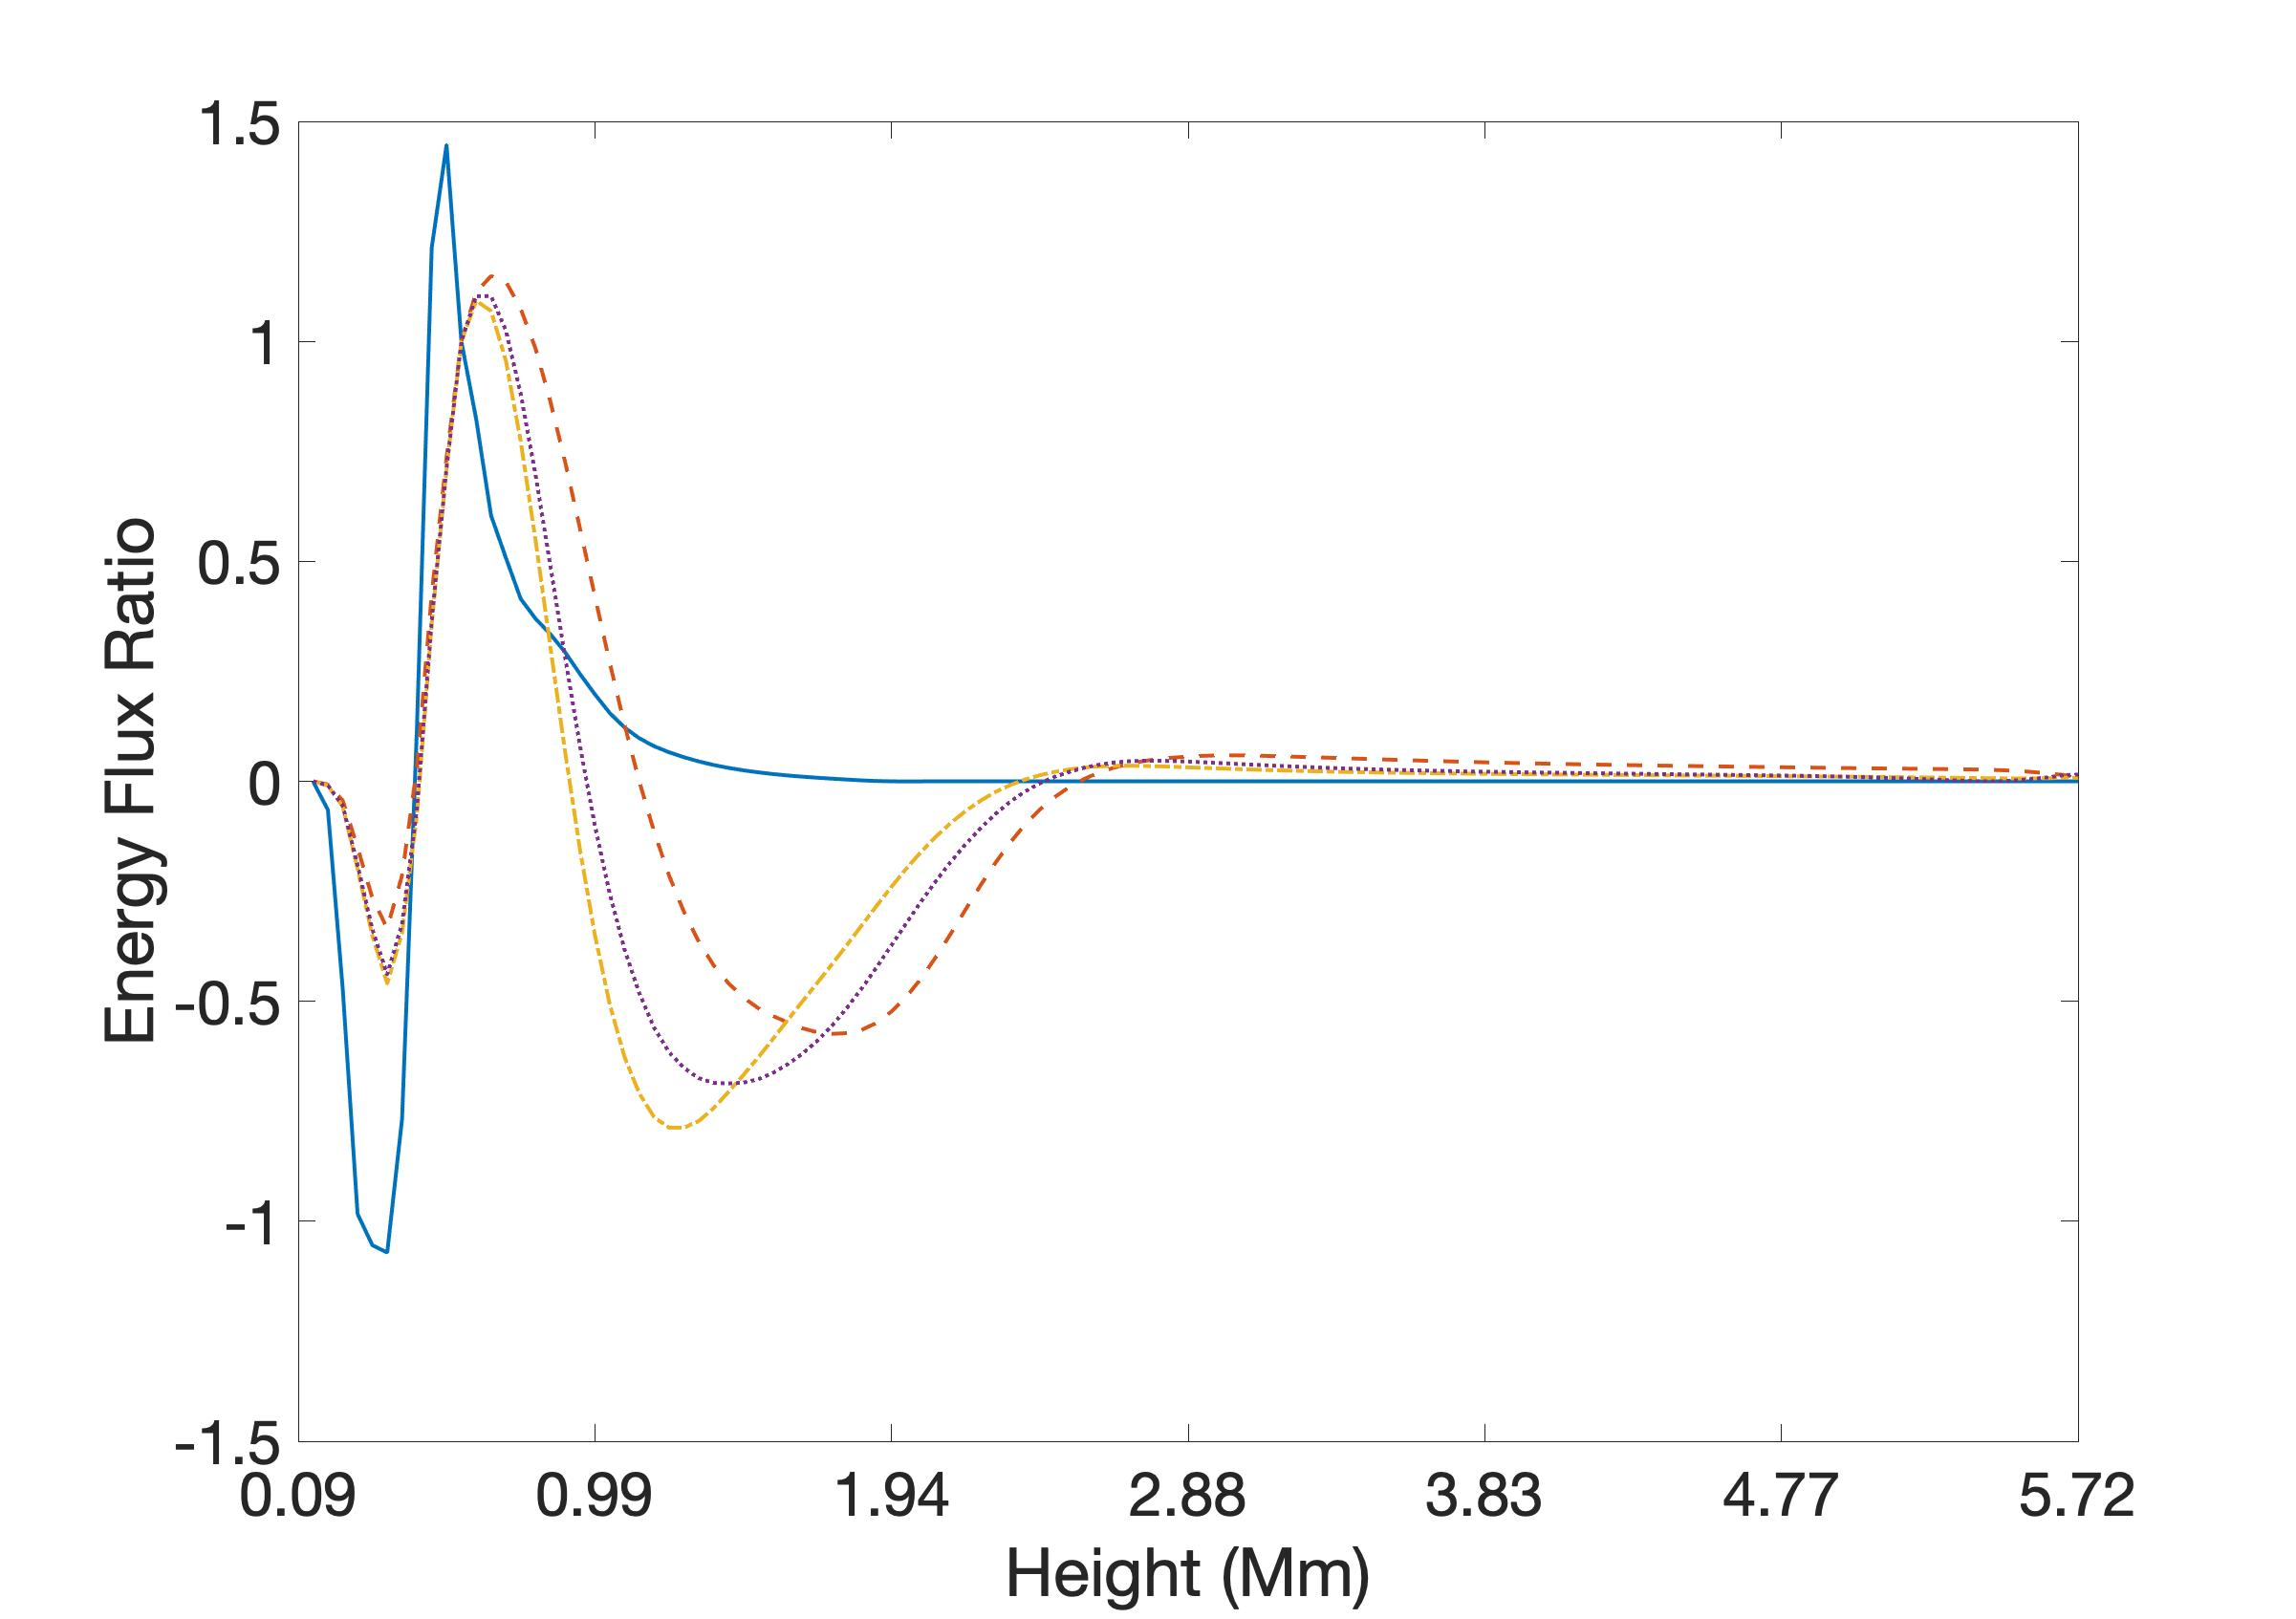
\includegraphics[width=11.5%10.5 %MDPI: figure size increased. Please confirm. MKG confirmed 
cm]{energyfluxratio.jpg}
    \caption{\hl{The ratio} %MDPI: 1. Please change the hyphen (-) into a minus sign ($-$, "U+2212"). e.g., "-1" should be "$-$1".
     %   2. Please increaase the size of the axes labels and the values on the axes. Almost innvisible otherwise. MKG font size increased
 of the integrated energy flux ratio for different values of the field: 
 %blue 0~G, orange 50~G, purple 75~G and red 100~G.\label{fig9}}
 \hl{0~G (blue),} 50~G (orange), 75~G (purple), and 100~G (red). %MDPI: first the values as the sentence says it.
\label{fig9}}
\end{figure}
\unskip



%\begin{figure}
%    \label{obs}
%    \centering
%    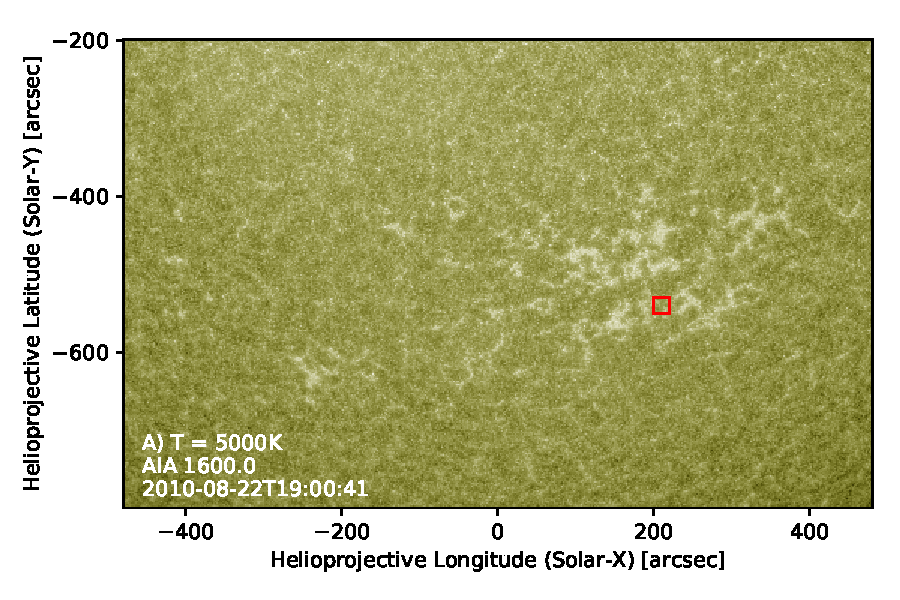
\includegraphics[scale=0.5]{obs_data.pdf}
 %   \caption{ The selected area from the start of the investigate time series at 18:00 UT on 22 August 2010. The area is indicated by red rectangle. The size of the selected area is 50 pixels.}
%\end{figure}

\section{Frequency~Analysis}

 We analysed the temporal behaviour of the numerical results, outlined in the previous section. %The~top panel of 
Figure~\ref{fig10} \hl{(top)} %MDPI: no "panel". Here and elsewhere below. 
shows a vertical slice of %$Bz$
 \highlighting{$B_z$} %MDPI: corrected. Please confirm. 
over time.  The~data are based on the simulation with the initial magnetic field configuration with a maximum value of $100$~G. 
 %The~vertical axis represents the height in Mm and the horizontal axis is the time dimension, measured in seconds. %MDPI: unnecessary, figure labels says it all. 
 \hl{From}~this two-dimensional plane, five layers were selected, representing different heights in the solar atmosphere. 
The~layers are indicated by the horizontal grey lines.   %The~middle panel of 
Figure~\ref{fig10} \hl{(top)} 
displays the temporal variation of the selected layers, indicated by different grey shade colours. 
A %n~
\hl{fast Fourier transform %MDPI: No undefined abbreviations even known or listed in the Abbreviations table.
(FFT)} was applied (\hl{see} %the lower panel of 
Figure~\ref{fig10} \hl{(bottom)}) 
 for investigating any oscillatory behaviour in the analysed signal. A~significant 
oscillatory pattern was found with frequency range of $3.75$--$4$~mHz, corresponding to a period range of $4.2$--$4.4$ min. 
A~slight frequency variation is also recognisable. The~different layers in height tend to feature variations in the peak positions 
identified from the FFT analysis. An~FFT was also performed based on the other simulations with different initial magnetic field 
configurations (with a maximum value of $0$~G , $50$~G,  $75$~G  and $100$~G). These investigations all showed similar oscillatory behaviour.  
Figure~\ref{fig11} features the same analysis as Figure~\ref{fig10}; however, the~study features a vertical slice of 
 %$Vz$ 
\highlighting{$V_z$} %MDPI: please confirm. MKG confirmed
over time. The~analysis shows similar properties as the data based on a vertical slice of 
\highlighting{$B_z$.}
%$Bz$.
 
 \begin{figure}[H]
   % \centering
    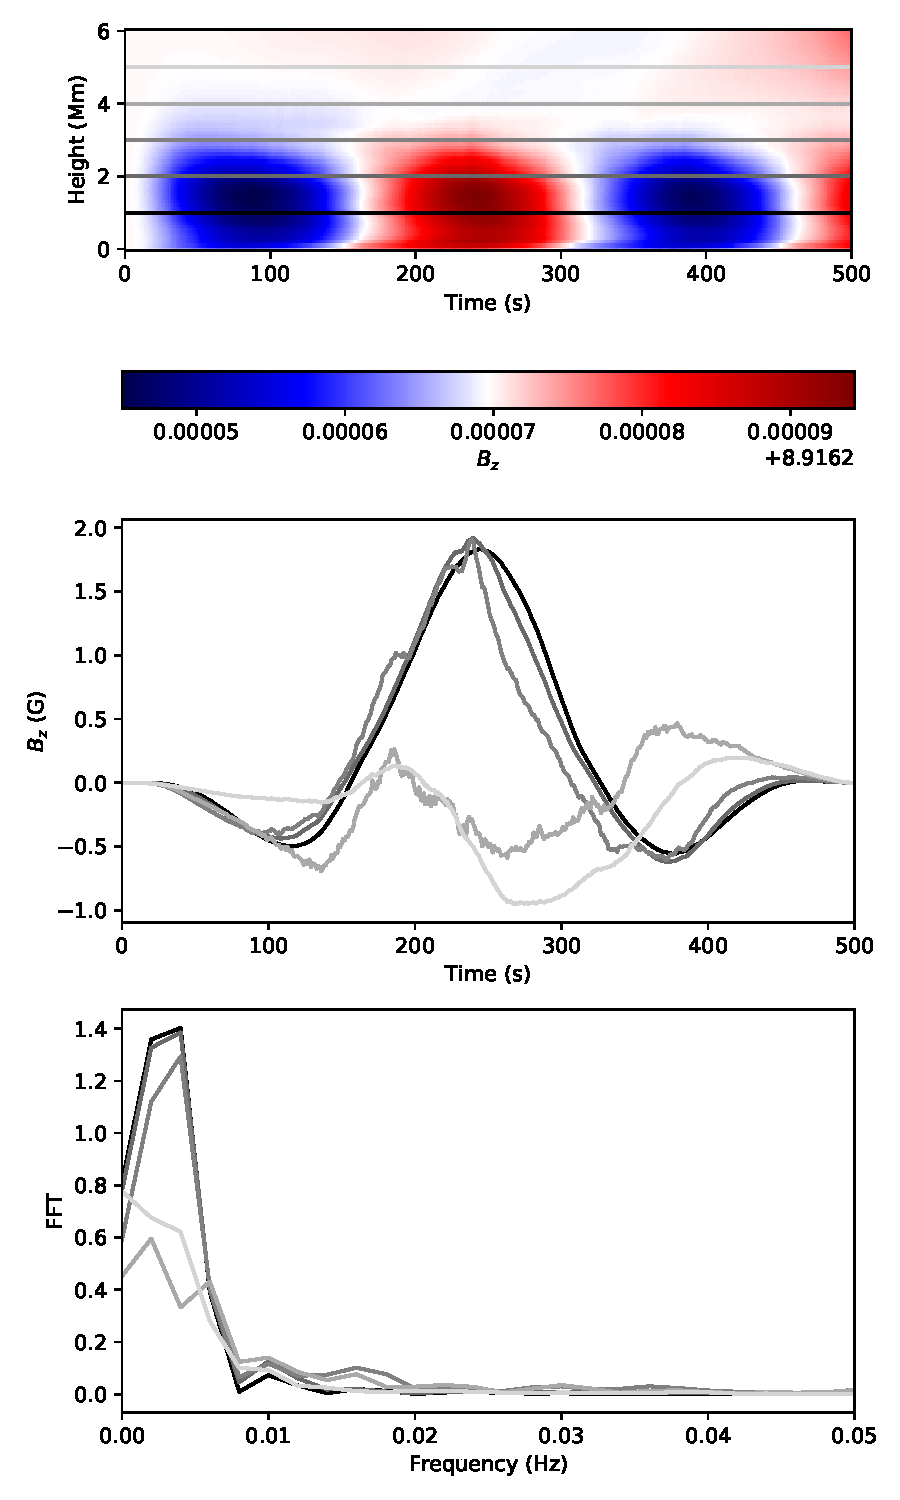
\includegraphics[width=9%8
.5cm]{fft_sim.pdf}
    \caption{\hl{Temporal} %MDPI: the size of the figure increased to make it better visible. Please confirm. Same for Fig. 11. MKG confirmed  
analysis of $B_{z}$ vertical slices at $2$ \hl{Mm:} \highlighting{({\bf top})} %. The~top panel shows 
the selected vertical slices, indicated by gray 
\highlighting{colours;  ({\bf middle})} %. The~middle panel demonstrates 
the obtained signal after applying a Hanning window \highlighting{function; and ({\bf bottom})} %. The~bottom panel shows 
the result of the \hl{fast Fourier transform  
(FFT)} analysis based on the 5~selected vertical $B_{z}$ slices.\label{fig10}}
\end{figure}

\begin{figure}[H]
   % \centering
    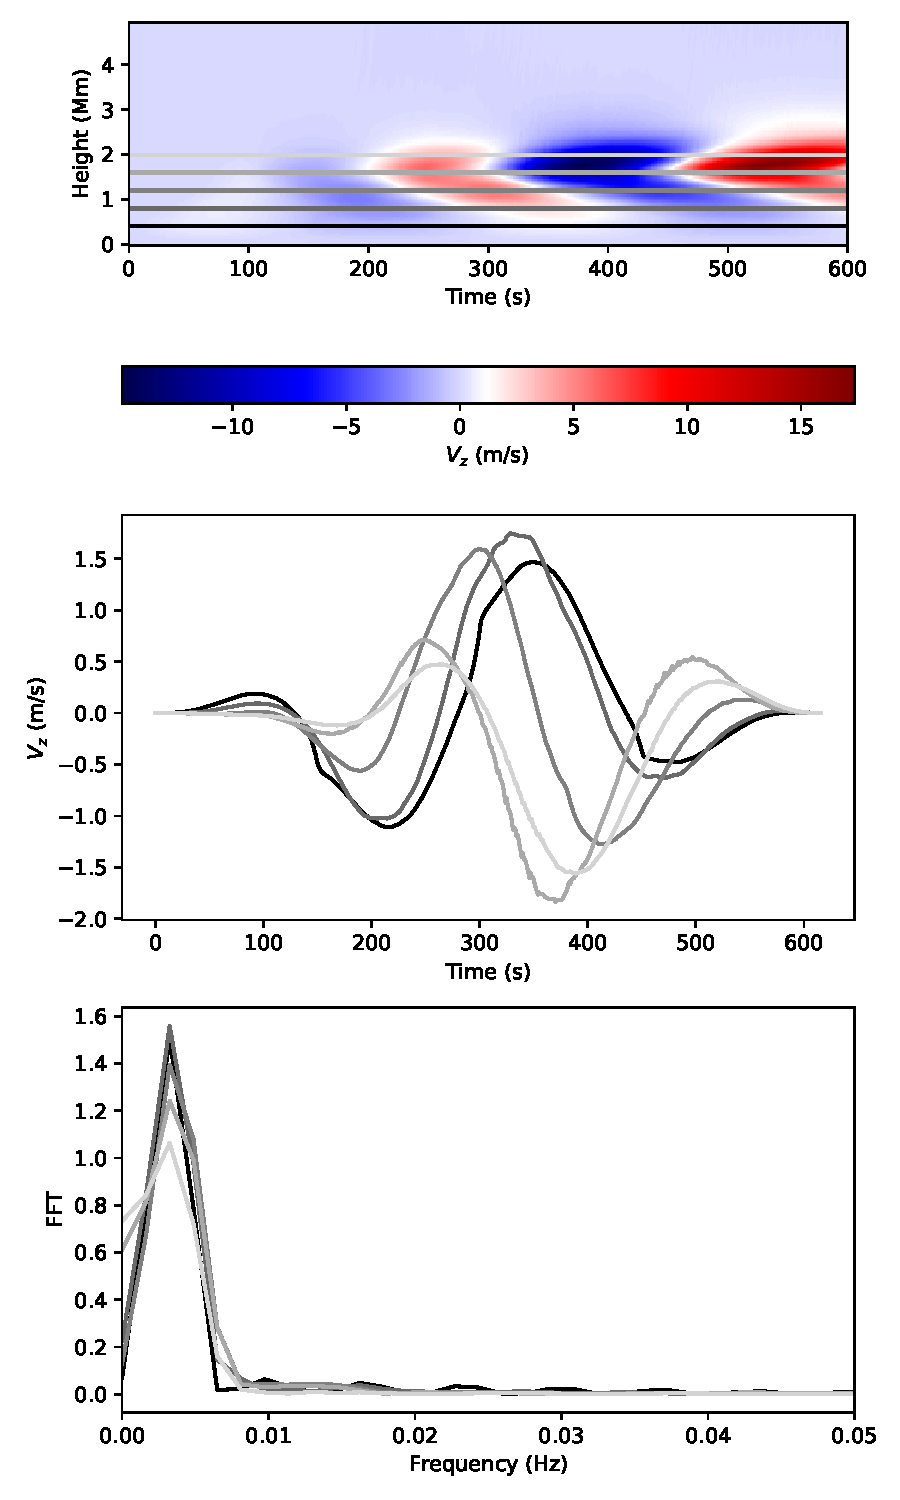
\includegraphics[width=9%8
.5cm]{fft_sim2.pdf}
    \caption{Temporal analysis of $V_{z}$ vertical slices at $2$~\hl{Mm:} \highlighting{({\bf top})} %.  The~top panel shows 
 the selected vertical slices, indicated by gray \highlighting{colours;  ({\bf middle})} %. The~middle panel demonstrates 
 the obtained signal after applying a Hanning 
window \highlighting{function; and ({\bf bottom})} %. The~bottom panel shows 
the result of the FFT analysis based on the $5$~selected vertical $V_{z}$ slices.
\label{fig11}}

\end{figure}
%\unskip


With the objective of confirming the obtained oscillatory behaviour, temporal analysis for the observational \hl{data}\cite{Pesnell2012}\cite{Lemen2012} %MDPI: please add the reference. MKG done 
was performed. We investigated intensity oscillations in the solar atmosphere observed by 
SDO/AIA  \hl{(Atmospheric Imaging Assembly).} 
The~passbands 1600 {\AA}, 1700 {\AA}, 304 {\AA}, 171 {\AA} and 193 {\AA} were selected because our simulation mainly focused on the lower atmospheric regions, i.e.,~photosphere, chromosphere and low corona. The~cadence of images is 24 s; therefore, it was suitable for studying relatively high-frequency oscillations such as the obtained $4$~mHz.

The initial magnetic field configuration of our model is a standing magnetic tube, passing through the chromosphere and the lower corona. 
The~selected area contains a small sunspot (e.g., a~solar pore), presumably featuring similar magnetic structure as our simulation. The~size 
of the investigated area covers 50 pixels in total between 18:00 UT to 20:00 UT on 22 August 2010. The~obtained time series shows 
non-stationary behaviour; therefore, the~observed linear trend is removed by taking the first difference $\Delta  y_{t}$ of the data. 
The~first difference is defined as the difference between consecutive observations $y_{t}$ and $y_{t-1}$. Furthermore, the~times series is 
also normalised by applying standard scores (\highlighting{$Z$}-scores), %MDPI: math mode, please confirm.
defined by 
\begin{equation}
	Z_{i} = \frac {T_{i} - \overline{T}}  {\sigma(T)},
	\label{z_score}
\end{equation}
where, the~parameter $\overline{T}$ is the mean of the time series and the parameter $\sigma(T)$ is defined as the standard deviation of the data. 
 %The~top panel of 
Figure~\ref{fig12} %MDPI: clear enough from the captions and axes labels. 
\hl{demonstrates} the trend removed and normalised time series \highlighting{($Z$-scores)} %MDPI: clarifies.
%. The~lower panel of {Figure~\ref{fig11}  
\hl{and shows} %MDPI: clear enough from the captions and axes labels. 
the result of the applied FFT technique. The~dashed line is the significance level ($3 \sigma$) which was calculated using a 
Monte Carlo method. The~original data showed red noise signature which transformed to blue noise after differentiating the data. 
We have generated 1 million blue noise \highlighting{signatures, $N_{b}$,} and calculated the standard \highlighting{deviation, 
$\sigma(N_{b})$,} 
and the 
\highlighting{mean, $\overline{N_{b}}$,} %MDPI: the commas added as the definiions introduced. 
of the simulated noise, providing our significance level $S$:
\begin{equation}
    S = \overline{N_{b}} + 3 \sigma(N_{b}).
\end{equation}

\begin{figure}[H]
   % \centering
        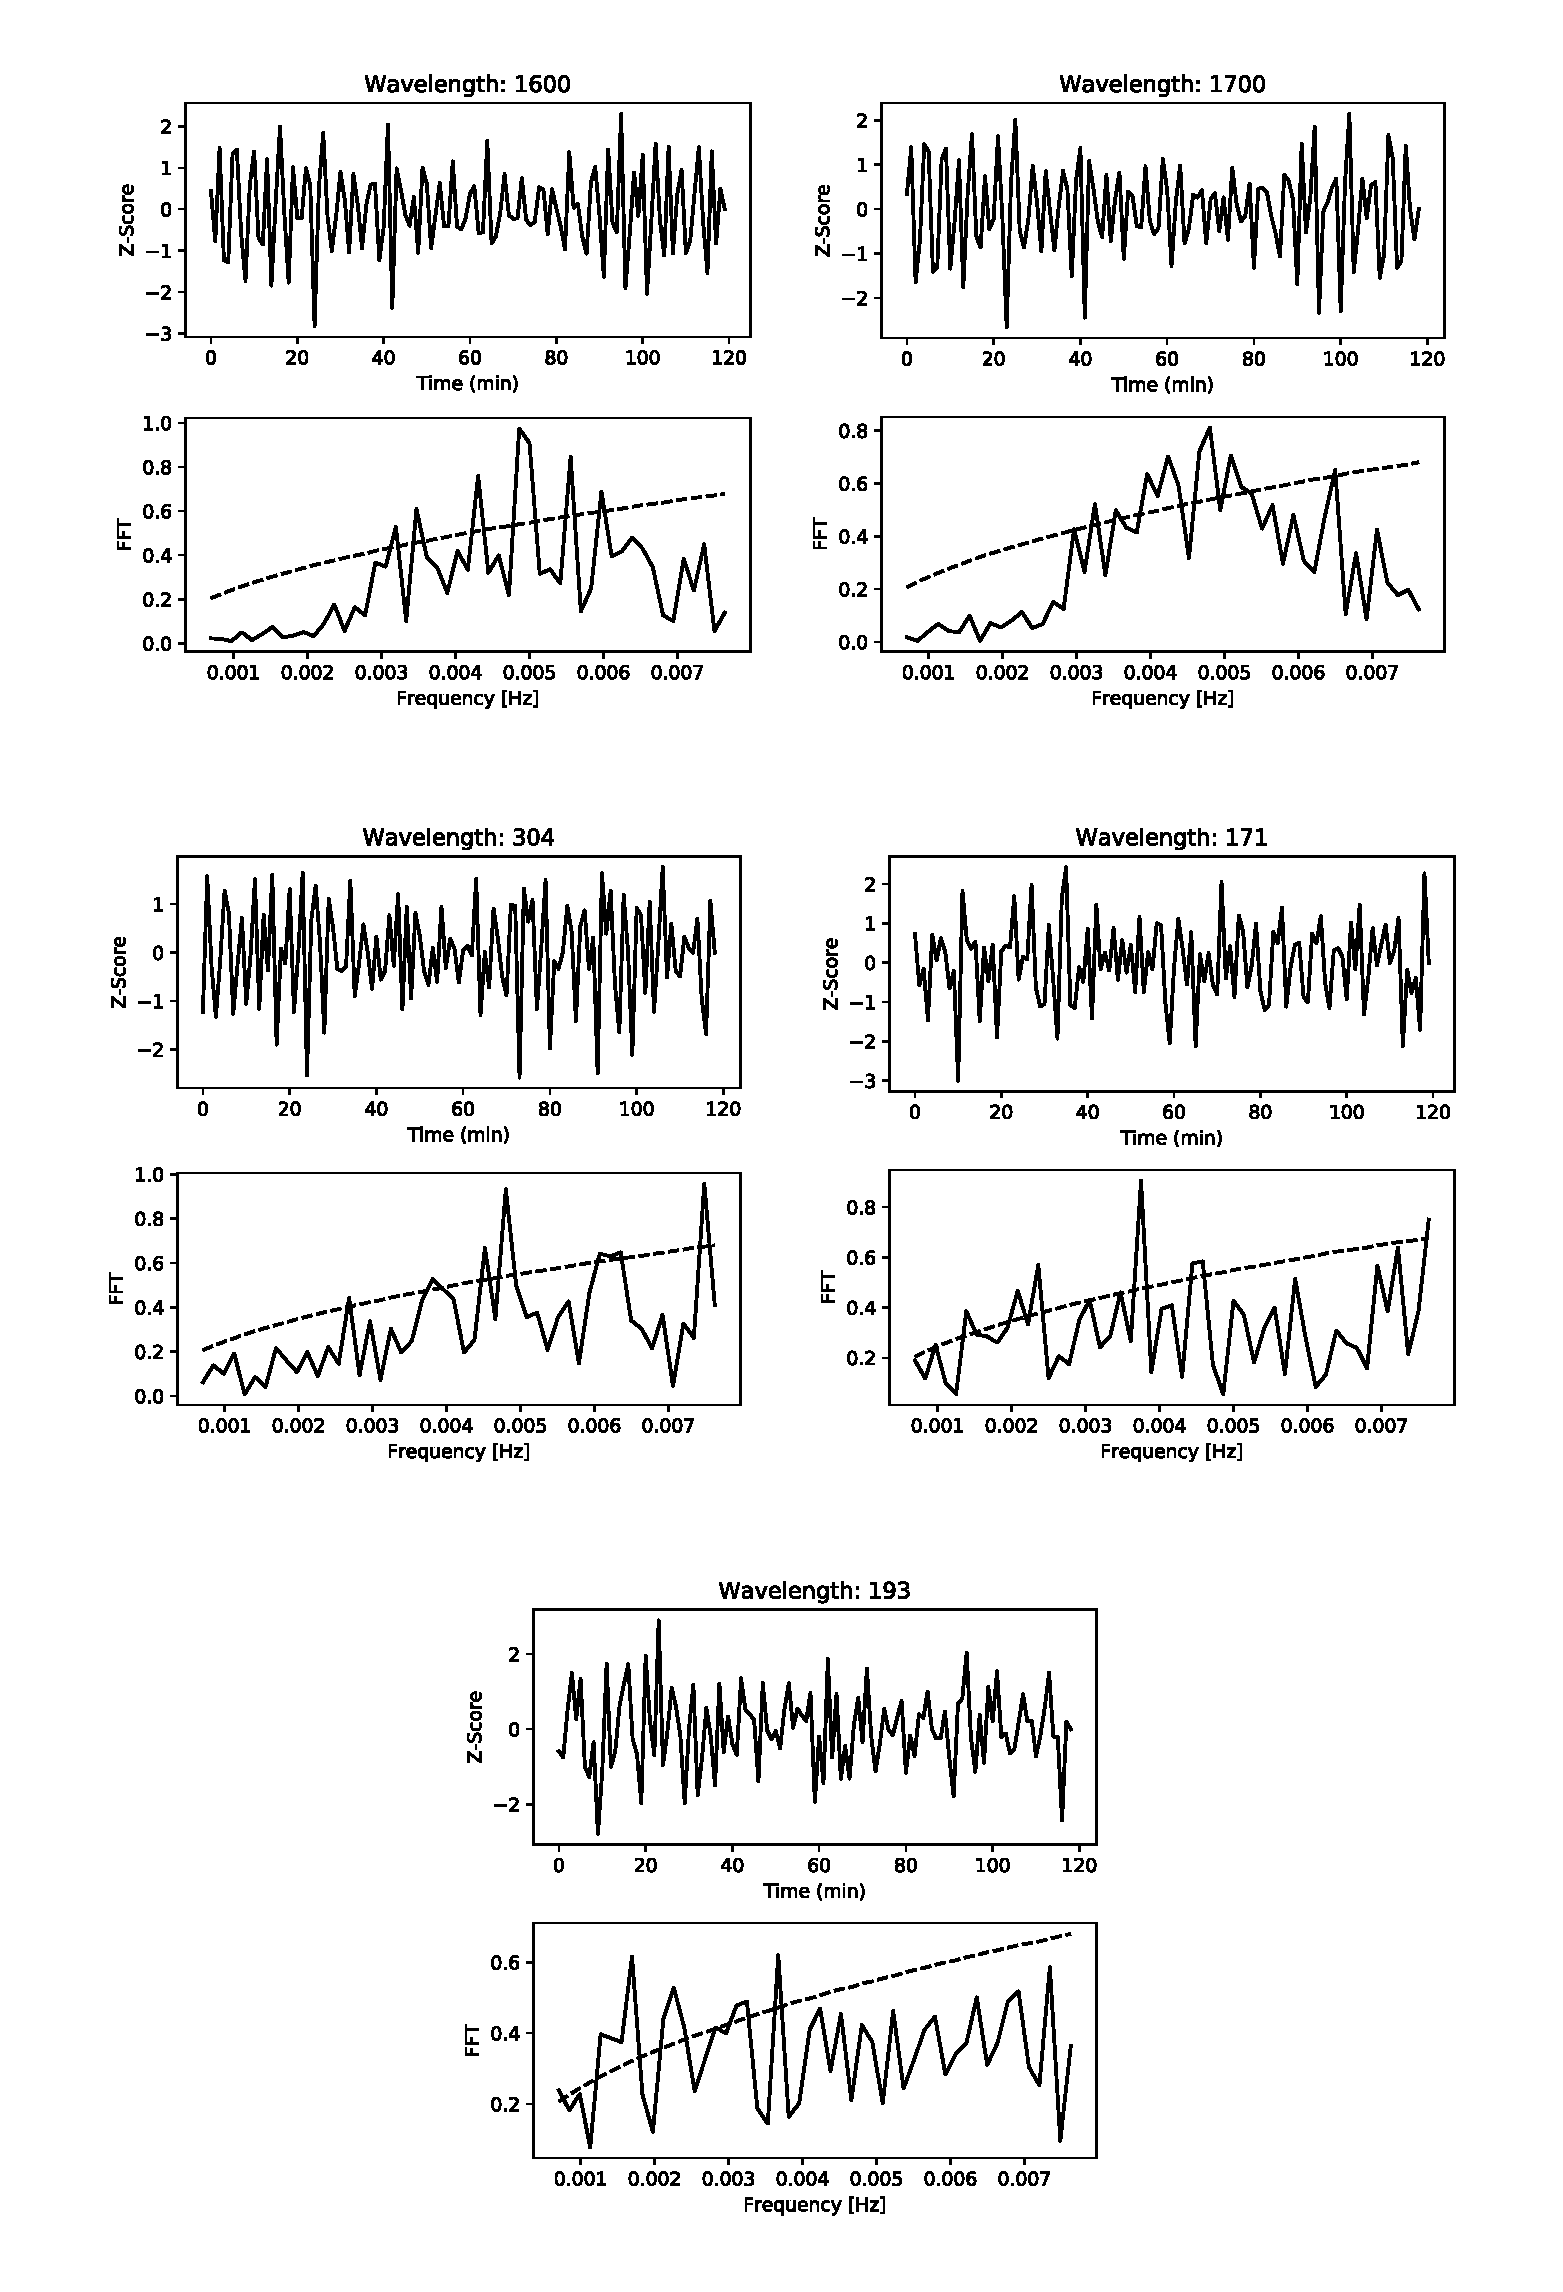
\includegraphics[scale=0.55]{QS_FFT.pdf}
    \caption{Temporal analysis of the intensity of a 50-pixel large area based on %AIA
\hl{the Atmospheric Imaging Assembly} 
 1600 {\AA}, 1700 {\AA}, 304 {\AA}, 171 {\AA} and 193 {\AA} \hl{data} %MDPI: please add the reference. 
between 18:00 UT to 20:00 UT on 22 August 2010. 
 \hl{The} %~upper panels show the temporal
 variation of the \highlighting{($Z$-score)} 
(de-trended by first difference and normalised pixel intensity data) \hl{and} %. The~lower panel shows 
the FFT of the 
analysed observational~data \hl{are shown as indicated.}
\hl{The dashed line} indicates  the significance level of 3 standard deviation calculated using a Monte Carlo method. %MDPI: added, otherwise unclear. Please consider. MKG OK
\label{fig12}}
\end{figure}



The results of the analyses are summarised in Table~\ref{tab3}. A~significant period is found with a frequency range of 3.5--4.2 mHz , corresponding a period range of $4.7$--$4$ min, which is close to the period found in simulation data. Another significant peak ($5$ mHz) is found with a period around $3$ min, which may be an indication of another global oscillation.  This randomly selected region in the solar surface suggests that the observed oscillation is a global~phenomenon.


\begin{table}[H]%\label{qsfrequencies}
\caption{The table shows observed \hl{frequencies} 
%(Hz) %MDPI: clear from teh Table.  
 for the 
 %Quiet
 \hl{quiet}  
Sun between 18:00 UT to 20:00 UT on 22 August \hl{2010,} %MDPI: please add the reference for the data. 
the~frequencies have been identified from the temporal analysis of a 50-pixel large area based on different AIA bands. Significant peaks around 5 min (0.0033 Hz) appear in bold~type.\label{tab3}}
%\label{FrequenciesQS}
%\centering
\newcolumntype{C}{>{\centering\arraybackslash}X}
\begin{tabularx}{\textwidth}{C C C C C}
\toprule
\textbf{1700 {\AA}}     &  \textbf{1600 {\AA}}   & \textbf{304 {\AA}}     & \textbf{171 {\AA}}     & \textbf{193 {\AA}}    \\
\midrule
{\bf 0.00332}  & 0.00311       & 0.00269       &  0.00141      & 0.00168      \\
%\midrule
0.00391	       & {\bf 0.00352} & {\bf 0.00382} & 0.00207       & 0.00227      \\
%\midrule
0.00423        & 0.00432	   & 0.00451       & 0.00238	   & {\bf0.00318} \\
%\midrule
0.00470        & 0.00488       & 0.00480	   & {\bf 0.00375} & 0.00369      \\
%\midrule
0.00512        & 0.00557       & 0.00619	   & 0.00456       & -            \\
%\midrule
0.00643	       & 0.00599	   & 0.00742       & 0.00762	   & -            \\

\bottomrule
\end{tabularx} 

\end{table}
\unskip




\section{Discussion}
Whilst many studies focus on local wave phenomena, the~simulations and observational analysis reported here are attempting to address the global oscillations of the solar atmosphere from the photosphere into the low corona. These ubiquitous oscillations result in a small but detectable leakage of energy from the chromosphere  into the coronal regions of the solar atmosphere. It is worth noting that this energy may not be adequate to heat these regions to the observed temperatures. However, addressing the 
 %well-
 \hl{known}   
solar atmospheric plasma heating is not the main concern of this paper. Its purpose is to show that these global oscillations are present, and just like in the inner regions or for coronal loops, they may be explored for~magneto-seismology.

Early theoretical studies   considered wave propagation in idealised magnetic slab structures and demonstrated the fundamental conditions for  
 %magnetohydrodynamic (MHD) 
 \hl{MHD} %MDPI: already defined. 
wave propagation~\cite{Roberts1981a,Roberts1981b}. These models were soon advanced to cylindrical magnetic structures and addressed 
%the conditions under 
the different types of MHD waves sustained under the conditions of the solar corona~\cite{EdwinandRoberts1983}.  Investigation of the propagation of magnetoacoustic oscillations in an isothermal atmosphere with a vertical magnetic field resulted in the prediction of small frequency shifts of solar global internal or acoustic oscillations, see, e.g.,~\cite{Hindman1996}. The~analysis was unable to demonstrate the absorption of MHD waves,  for~example as observed in sunspots. Many of these  earlier studies  focused on the effect of magnetic flux tubes on wave propagation and neglected gravitational stratification. Much effort has been made to understand the role of solar atmospheric oscillations in coronal heating. Such modelling has ranged from one dimensional models modelling radiative energy loss to %Please check intended meaning is retained
  taking into account two fluid models of the plasma. Further work investigated the influence of vertical fields on a variety of modes, including $p$-mode oscillations in an isothermal stratified atmosphere~\cite{Hasan1992}. In~the limit of weak fields these results were used to analyse the spectrum of the modes of oscillation for the stratified~atmosphere.



The  \hl{review} %of~ %MDPI: clear enough.
\cite{Khomenko2013} considered localised wave phenomena and variation in different magnetic structures of the 
 %Quiet
 \hl{quiet}  
Sun. For~example, in~the close proximity of the magnetic network elements, the~longer 5-minute modes propagate efficiently to the chromosphere. The~3-minute modes propagate from the photosphere to the chromosphere in the network cell interiors for restricted regions of the network and internetwork.  Observations show that the 3-minute modes exhibit enhancement in both the photosphere and the chromosphere, whereas the power of the 5-minute modes increases significantly in the chromosphere. These power enhancements are known as 
''halos'' and have been %widely
 \hl{well}  
reported~\cite{Kontogiannis2010}. 
%Dicussion section where they clearly state what is new in their simulations and compare their findings against simular efforts if there are any. 
In contrast, the~work reported here is an extension of an earlier study representing photospheric $p$-mode oscillations using different point drivers~\cite{Malins2007}. These studies demonstrated  the generation of surface waves, structures in the transition zone and identified the effect of cut-offs induced by the stratified  solar atmosphere. The brief overview in Section~\ref{sec2} identified the physical phenomena of leaking energy into the lower solar atmosphere and the resulting oscillatory behaviour~there.

An initial study of global oscillations in a highly gravitationally stratified atmosphere looked at the variation of energy leakage with different modes of oscillation of an extended driver~\cite{Griffiths2018b}. The~investigation addressed an observational study indicating the ubiquitous nature of intensity oscillations. The~power spectra presented in 
 %the first figure 
\hl{Figure~1} %MDPI: please confirm the meaning retained. MKG confirmed thank you 
of~\hl{Ref.} 
\cite{Griffiths2018b} exhibit a variation of propagation characteristics at different levels within the solar atmosphere and within different regions such as coronal holes, 
the~\hl{quiet} 
 %Quiet 
Sun and active regions. The~power spectra indicate a preponderance of long-period 5-minute waves with frequencies in the range of 1.5--5 mHz. Furthermore, observed are the distinctive peaks for the short-period 3-minute waves (with frequencies in the range of 5--8 mHz). The~power spectra exhibit  peaks in much longer period ranges, for example 12-minute waves  (frequencies in the range 1.1--1.5 mHz)  and 16-minute waves (frequencies 1--1.1 mHz). For~the 
 %Quiet 
\hl{quiet} 
Sun regions the 5-minute modes are stronger at photospheric levels and diminished higher up in the corona; there is a small peak for the data from the AIA passband at 211 {\AA} corresponding to the corona at 2.0 MK.  The~computational results presented here corroborate the suggestion of~\cite{Didkovsky2013} of the existence of global oscillations in the solar corona. The~suggestion of small energy deposition events was indicated by~\cite{Ireland2015} in their study of power spectra of the solar corona. They suggest that this is the result of the summation of energy deposition events in the solar~atmosphere.



 



The remaining study 
%Please check intended meaning is retained
 focused on global oscillations of the solar atmosphere and employing extended drivers to emulate a driving \hl{p}-mode oscillation. The initial work with a hydrodynamic model was extended into an idealised model of a typical solar pore. Further, as~a test of ubiquity, the~observational analysis has been for randomly selected regions and the Fourier analysis for the observational results has been compared to a similar analysis for the simulated~feature.  








\section{Conclusions}

In this paper, we have presented results for a series of MHD simulations of an extended oscillator at the base of a simple model solar atmosphere. A~comparison with observational data provides a unique insight into the nature of  global oscillations in the upper solar atmosphere caused by the ubiquitous \hl{p}-mode oscillation. It was found that the oscillations are enhanced by a vertical magnetic field. Although~the observational data suggest that the global atmospheric oscillations are detectable through oscillations in intensity, the~small energy leakage is not sufficient for heating of the solar corona; this is supported by the results of the~simulations.

We  have successfully extended the initial hydrodynamic model of global oscillations to test how the SMAUG~\cite{Griffiths2015} code works when our model atmosphere includes an initially symmetric and uniform magnetic field. Accelerated MHD codes such as SMAUG are a key requirement for simulations of magnetic and highly stratified plasma which are run for long time periods, for~example, for~models of the solar global oscillations. As~attempts are made to model large scale and more complex regions of the solar atmosphere, multiple graphical processing units will be~required.

The simulations with an extended driver show that the observed  solar atmospheric global oscillations are enhanced by regions with a vertical magnetic field. Investigation of the energy flux propagation results are indicative of the enhanced propagation of energy with increasing magnetic fields, but this is not sufficient to result in significant solar coronal heating. The~analysis suggests that the energy propagation is by magnetosonic modes. Due to the steep density changes around the transition region, slow and fast magnetosonic modes are responsible for reflecting some energy back to the chromosphere and the~photosphere.  

The FFT analysis of the simulated data demonstrated the presence of oscillations with periods in the range of 4.2--4.4 min. This arose for both the hydrodynamic case and the case with a magnetic field of 100~G. In~ the latter case there was some additional structure for the FFT analysis. There is a clear variation of the oscillation frequency around the 5~min period of the~driver. 

It is interesting that there is a similarity between the FFT analysis  of simulations and observations for different solar features, for~example for the 
 %Quiet 
 \hl{quiet} 
Sun or for regions with pores. The~results, derived from intensity time series of SDO images, also exhibit a significant variation of the oscillation frequency from the period of the global 5-minute oscillation.  The~frequency variation is larger than would be expected from  simple (e.g., linear) theory. Such frequency variations may be attributed to additional elasticity in the solar atmosphere resulting from the presence of a magnetic field, from~non-linear processes or from the artefacts of the observational method. This  may be understood in part by referring to 
 %the work of
\hl{Ref.}~\cite{Campbell1989}; however, in~their model the magnetic field was horizontal. An~explanation based on 
 the %work 
 \hl{study} of~\hl{Ref.}
\cite{Hindman1996} does not seem to explain the size of the frequency variations found in the~simulations.

 
  
  

%REFEREE COMMENT
% Line 269. It is misleading mentioning the frequency shifts obtained by Hindman~et~al. (1996) because the current work does not have enough frequency resolution to detect such shifts. In addition, the physical mechanisms behind these shifts is not explained in the paper.
 
% Section~9. How long is the time series used in this work? Have the simulations achieve the stationary regime?
%Have the authors taken the part fo the time series in the stationary regime for the Fourier analysis? From what is shown in Figures like 9 and 10, this does not seem to be the case. Therefore, I do not understand how any conclusions about possible frequency shifts can be made from a time series of about 600 duration. This time series fits 2 wave periods, and part of the time is not in the stationary regime.
 
%END OF REFEREE COMMENT
Care must be taken with the measurement of the simulated frequency variation, and further work is required to provide more insight into the different mechanisms. An~example could be a result of the superposition of waves arriving at different heights and times, such a mechanism allows for the spatio-temporal variation of the   magnetic field. Improved boundary conditions handling reflections from the upper boundary  will be required to run simulations for much longer time intervals and with inclined magnetic fields. A~further consideration may be a comparison of the results from the vertical tube with a model which is an improved representation of a solar pore~\cite{Simon1970,Cameron2007}.

It is encouraging that the results presented here are consistent with the behaviour exhibited by earlier \hl{studies}.
 %work. 
There is an issue that due to the extended nature of the driver, the~amplitudes are responsible for delivering vast quantities of energy into the solar atmosphere inducing extremely large shocks and result in a numerically unstable system~\cite{Santamaria2015}. Significant improvements to the comparisons presented in this paper are expected with the  recent 
 %work 
 \hl{study} of \hl{Ref.}~\cite{Kostogryz2021}. Here, using the ADIPLS \hl{code} %MDPI: clear enough.
%of
\cite{Christensen-Dalsgaard2008}, a model of the intensity 
perturbations 
using a VALIIIc solar atmosphere model with radiative transfer was used to simulate the intensity oscillations perturbed by the solar global oscillations. As~described 
in~\hl{Ref.} 
\highlighting{\cite{Rast2016}}%MDPI: Refs. [57], [58], and [59] are missing. Please add and rearrange all the references to appear in numerical order.
, more sensitive observations with instruments such as DKIST \hl{(the Daniel K. Inouye Solar Telescope)} % 
may enable further constraints on the range of theoretical models. 
%e.g., cite reference Solar Physics Fedun et al. 2009 oscillatory response 3d solar atmosphere to leakage of photospheric motions








%%%%%%%%%%%%%%%%%%%%%%%%%%%%%%%%%%%%%%%%%%
%\authorcontributions{For research articles with several authors, a short paragraph specifying their individual contributions must be provided. The following statements should be used ``Conceptualization, X.X. and Y.Y.; methodology, X.X.; software, X.X.; validation, X.X., Y.Y. and Z.Z.; formal analysis, X.X.; investigation, X.X.; resources, X.X.; data curation, X.X.; writing---original draft preparation, X.X.; writing---review and editing, X.X.; visualization, X.X.; supervision, X.X.; project administration, X.X.; funding acquisition, Y.Y. All authors have read and agreed to the published version of the manuscript.'', please turn to the  \href{http://img.mdpi.org/data/contributor-role-instruction.pdf}{CRediT taxonomy} for the term explanation. Authorship must be limited to those who have contributed substantially to the work~reported.}
\vspace{6pt}
\authorcontributions{Conceptualisation, 
\hl{R.E.,} %MDPI: any preference of this order and not in the order of the author list? If no preference, please rearrange due to the author list here and below.
R.Z., N.G., \hl{M.K.} %MDPI: We revised M.B.K. to M.B., please confirm. MKG you mean to MK
 and M.G.; methodology, R.E.,
N.G. and M.G.; software, M.G. and N.G.; validation, M.G. and N.G.; formal analysis, R.E., M.G. and N.G.; writing---original draft preparation, M.G.; writing---review and editing, R.E., M.G., N.G., 
\hl{M.K.};  
visualisation, M.G. and N.G.; preparation of Figure~\ref{fig1},
 % and helpful discussion,  %MDPI: removed as is assumed by default. Please confirm.
 \hl{M.K.};  
supervision, R.E.; funding acquisition, R.E. All authors have read and agreed to the published version of the~manuscript.
}

\funding{This research was funded by the UK, Science and Technology Facilities Council (STFC)
\hl{(grant number ST/M000826/1).} 
R.E. acknowledges the support received from the the Royal Society (UK).
R.E. also acknowledges support from the European Union's Horizon 2020 research and innovation programme under the grant agreements no.
739500 (PRE-EST project) and no. 824135 (SOLARNET project).
 \hl{M.K.}
is grateful to ST/S000518/1, PIA.CE.RI. 2020-2022 Linea2, CESAR 2020-35-HH.0, and~UNKP-22-4-II-ELTE-186 grants \hl{(UK)}. %MDPI: please confirm or indicate countries for each if different. MKG confirmed
}

\dataavailability{\hl{The data used can be obtained in the references cited and on request from the corresponding author}}. %MDPI: please confirm.

%MKG confirmed
%{\color{red}{We always 
%encourage the authors indicating if the results reported can be obtained upon request. Please say so if applicable.}}
%MDPI: In this section, please provide details regarding where data supporting reported results can be found, including links to publicly archived datasets analyzed or generated during the study. Please refer to suggested Data Availability Statements in section ``MDPI Research Data Policies'' at \url{https://www.mdpi.com/ethics}. If the study did not report any data, you might add ``Not applicable'' here.

\acknowledgments{The authors thank P.H. Keys for providing the wavelet tools to analyse the related SDO \hl{data.} %MDPI: the grant parts moved to the Funding section. Please consider. 
%, the~Science and Technology Facilities Council (STFC) of the UK for the support they received (grant number ST/M000826/1).  
%R.E. acknowledges the support received from the the Royal Society (UK). 
%R.E. also acknowledges support from the European Union's Horizon 2020 research and innovation programme under the grant agreements no. 
%739500 (PRE-EST project) and no. 824135 (SOLARNET project). 
%{M.B.K.} is grateful to ST/S000518/1, PIA.CE.RI. 2020-2022 Linea2, CESAR 2020-35-HH.0, and~UNKP-22-4-II-ELTE-186 grants. 
R.E. and 
 \hl{M.K.}  
are also grateful to \hl{NKFIH}\hl{, National Research and Innovation Office}
(OTKA, \hl{the Hungarian Scientific Research Fund}, grant No. K142987), Hungary,  for enabling this research.
We acknowledge IT Services at The University of Sheffield for the provision of the High Performance Computing~Service.}


%% To help institutions obtain information on the effectiveness of their 
%% telescopes the AAS Journals has created a group of keywords for telescope 
%% facilities.
%
%% Following the acknowledgments section, use the following syntax and the
%% \facility{} or \facilities{} macros to list the keywords of facilities used 
%% in the research for the paper.  Each keyword is check against the master 
%% list during copy editing.  Individual instruments can be provided in 
%% parentheses, after the keyword, but they are not verified.

%%\vspace{5mm}
%%\facilities{HST(STIS), Swift(XRT and UVOT), AAVSO, CTIO:1.3m,
%%CTIO:1.5m,CXO}

%% Similar to \facility{}, there is the optional \software command to allow 
%% authors a place to specify which programs were used during the creation of 
%% the manusscript. Authors should list each code and include either a
%% citation or url to the code inside ()s when available.


%\conflictsofinterest{Declare conflicts of interest or state ``The authors declare no conflict of interest.'' Authors must identify and declare any personal circumstances or interest that may be perceived as inappropriately influencing the representation or interpretation of reported research results. Any role of the funders in the design of the study; in the collection, analyses or interpretation of data; in the writing of the manuscript; or in the decision to publish the results must be declared in this section. If there is no role, please state ``The funders had no role in the design of the study; in the collection, analyses, or interpretation of data; in the writing of the manuscript; or in the decision to publish the~results''.} 
\conflictsofinterest{The authors declare no conflicts of interest. The~funders had no role in the design of the study; in the collection, analyses, or~interpretation of data; in the writing of the manuscript; or in the decision to publish the~results.} 
%%%%%%%%%%%%%%%%%%%%%%%%%%%%%%%%%%%%%%%%%%
\noindent
\highlighting{{\bf Software:} SMAUG, \citet{Griffiths2015}, SAC \citet{Shelyag2008},             
          VAC \citet{Toth1996}.} %MDPI: please move this to the main.text where appropriate.
%% Only for journal Encyclopedia
%\entrylink{The Link to this entry published on the encyclopedia platform.}

%\newpage
\abbreviations{Abbreviations} {The following abbreviations are used in this manuscript:\\

\noindent 
\begin{tabular}{@{}ll}
%MDPI & Multidisciplinary Digital Publishing Institute\\
%DOAJ & Directory of open access journals\\
%TLA & Three letter acronym\\
%LD & Linear dichroism
AIA & Atmospheric Imaging Assembly \\
\hl{DKIST} & the Daniel K. Inouye Solar Telescope\\
FFT & \hl{fast Fourier transform} \\
GPU & \hl{graphical processing unit} \\
MHD & \hl{magnetohydrodynamics} \\
SDO & Solar Dynamics Observatory \\
SMAUG & Sheffield \hl{magnetohydrodynamics accelerated using} GPUs \\
VAC & Versatile Advection Code \\
VALIIIc & Vernazza, Avrett and Loeser\\
\hl{1D,} 2D, 3D & one-, two-, three-dimensional

\end{tabular}
}

%%%%%%%%%%%%%%%%%%%%%%%%%%%%%%%%%%%%%%%%%%
\begin{adjustwidth}{-\extralength}{0cm}
	%\printendnotes[custom] % Un-comment to print a list of endnotes
	
	\reftitle{References}
	
	% Please provide either the correct journal abbreviation (e.g. according to the “List of Title Word Abbreviations” http://www.issn.org/services/online-services/access-to-the-ltwa/) or the full name of the journal.
	% Citations and References in Supplementary files are permitted provided that they also appear in the reference list here. 
	
	%=====================================
	% References, variant A: external bibliography
	%=====================================
	%\bibliography{your_external_BibTeX_file}
	
	%=====================================
	% References, variant B: internal bibliography
	%=====================================
	\begin{thebibliography}{999}
		
		\bibitem[Erd{\'e}lyi(2006)]{Erdelyi2006} Erd\'elyi, R. Magnetic coupling of waves and oscillations in the lower solar atmosphere: 
Can 
the tail wag the dog? \emph{Philos. Trans. R. Soc. A Math. Phys. Eng. Sci.} \textbf{2005}, \emph{364}, 351--381. https://doi.org/10.1098/rsta.2005.1703.
		
		\bibitem[Taroyan \& Erd{\'e}lyi(2008)]{Taroyan2008} Taroyan, Y.; Erd\'elyi, R. Global acoustic resonance in a stratified 
solar atmosphere. \emph{Sol. Phys.} \textbf{2008}, \emph{251}, 523--531. https://doi.org/10.1007/s11207-008-9154-3.
		
		\bibitem[Pint{\'e}r et al.(2007)]{Pinter2007} Pint\'er, B.; Erd\'elyi, R.; Goossens, M. Global oscillations in a magnetic 
solar model. \aap~\textbf{2007}, \emph{466}, 377--388. https://doi.org/10.1051/0004-6361:20041632.
		
		\bibitem[Mein and Mein(1976)]{Mein1976}Mein, N.; Mein, P.  \hl{Velocity waves in the quiet solar chromosphere}%MDPI: Newly added information by google, please confirm, same as refs 42,48,59.
		. \emph{Sol. Phys.} \textbf{1976}, \emph{49}, 231\hl{--248.} https://doi.org/10.1007/BF00162447.
		
		\bibitem[Schmieder \& Mein(1980)]{Schmieder1980} Schmieder, B.; Mein, N. \hl{Mechanical flux in the solar chromosphere. II. 
Determination of the mechanical flux}. \aap~\textbf{1980}, \emph{84}, 99\hl{--105.}
\hl{Available online:} \url{https://ui.adsabs.harvard.edu/abs/1980A%26A....84...99S/} (accessed on 18 March 2023).
		
		\bibitem[De Moortel (2009)]{deMoortel2009} De Moortel, I. Longitudinal waves in coronal loops. \ssr~\textbf{2009}, \emph{149}, 
65--81. https://doi.org/10.1007/s11214-009-9526-5.
		
		\bibitem[Banerjee et al. (2011)]{Banerjee2011} Banerjee, D.; Gupta, G.R.; Teriaca, L. Propagating MHD waves in coronal holes. \ssr~\textbf{2010}, \emph{158}, 267--288. https://doi.org/10.1007/s11214-010-9698-z.
		
		\bibitem[Mathioudakis et al.(2013)]{Mathioudakis2013} Mathioudakis, M.; Jess, D.; Erd\'elyi, R. Alfv\'en waves in the solar 
atmosphere. \ssr~\textbf{2012}, \emph{175}, 1--27. {\changeurlcolor{black}\url{https://doi.org/10.1007/s11214-012-9944-7}.} 
		
		\bibitem[Ruderman \& Erd{\'e}lyi(2009)]{Ruderman2009} Ruderman, M.S.; Erd\'elyi, R. Transverse oscillations of coronal loops. 
\ssr~\textbf{2009}, \emph{149}, 199--228. {\changeurlcolor{black}\url{https://doi.org/10.1007/s11214-009-9535-4}.}

 	\bibitem[Wang(2011)]{Wang2011} Wang, T. {Standing slow-mode waves in hot coronal loops: Observations, modeling, and coronal 
seismology}. \ssr~\textbf{2011}, \emph{158}, 397\hl{--419.}  https://doi.org/10.1007/s11214-010-9716-1.
		
		\bibitem[Auch{\`e}re et al. (2014)]{Auchere2014} Auchère, F.; Bocchialini, K.; Solomon, J.; Tison, E. Long-period intensity pulsations in the solar corona during activity cycle 23. \aap~\textbf{2014}, \emph{563}, A8. https://doi.org/10.1051/0004-6361/201322572.
		
		\bibitem[Jensen \& Orrall(1963)]{Jensen1963} Jensen, E.; Orrall, F.Q. Observational study of macroscopic inhomogeneities in the 
solar atmosphere. IV. Velocity and intensity fluctuations observed in the K line. \apj~\textbf{1963}, \emph{138}, 252\hl{--270.} 
 \hl{https://doi.org/10.1086/147631}
 %\hl{Available online:} \url{https://ui.adsabs.harvard.edu/abs/1963ApJ...138..252J/} (accessed on 18 March 2023). %MDPI: just in case, we give  the URL, as DOI link fails. Here ad below for APJ family. Please check.
		
		\bibitem[Banerjee et al.(2007)]{Banerjee2007} 		Banerjee, D.; Erd\'elyi, R.; Oliver, R.; O’Shea, E. Present and future 
observing trends in atmospheric magnetoseismology. \emph{Sol. Phys.} \textbf{2007}, \emph{246}, 3--29. https://doi.org/10.1007/s11207-007-9029-z.
		
		\bibitem[Erd{\'e}lyi \& Taroyan(2008)]{Erdelyi2008} Erd\'elyi, R.; Taroyan, Y. Hinode EUV spectroscopic observations of coronal 
oscillations. \aap~ \textbf{2008}, \emph{489}, L49--L52. https://doi.org/10.1051/0004-6361:200810263.
		
		\bibitem[Roberts et al.(1984)]{Roberts1984} Roberts, B.; Edwin, P.M.; Benz, A. On coronal oscillations. \apj~\textbf{1984}, \emph{279}, 857--865. 
\hl{https://doi.org/10.1086/161956.}
%\hl{Available online:} \url{https://ui.adsabs.harvard.edu/abs/1984ApJ...279..857R} (accessed on 18 March 2023).  		

		\bibitem[Verth et al.(2010)]{Verth2010} Verth, G.; Erd\'elyi, R.; Goossens, M. Magnetoseismology: Eigenmodes of torsional Alfv\'en 
waves in stratified solar waveguides. \apj~\textbf{2010}, \emph{714}, 1637--1648. https://doi.org/10.1088/0004-637x/714/2/1637.

 \bibitem[Zaqarashvili \& Murawski(2007)]{Zaqarashvili2007} Zaqarashvili, T.V.; Murawski, K. {Torsional oscillations of 
longitudinally inhomogeneous coronal loops}. \aap~\textbf{2007}, \emph{470}, 353\hl{--357.} https://doi.org/10.1051/0004-6361:20077246.
		
		\bibitem[Gyenge \& Erd{\'e}lyi(2018)]{Gyenge2018} Gyenge, N.; Erd\'elyi, R. Periodic recurrence patterns in X-Ray solar flare 
appearances. \apj~\textbf{2018}, \emph{859}, 169. https://doi.org/10.3847/1538-4357/aac109.
		
		\bibitem[{Gudiksen} et~al.(2011){Gudiksen}, {Carlsson}, {Hansteen}, {Hayek}, {Leenaarts}, and {Mart{\'{\i}}nez-Sykora}]{Gudiksen2011}		Gudiksen, B.V.; Carlsson, M.; Hansteen, V.H.; Hayek, W.; Leenaarts, J.; Martínez-Sykora, J. The stellar atmosphere simulation codeBifrost. \aap~\textbf{2011}, \emph{531}, A154. https://doi.org/10.1051/0004-6361/201116520.
		
		\bibitem[{V{\"o}gler} et~al.(2005){V{\"o}gler}, {Shelyag}, {Sch{\"u}ssler},
		{Cattaneo}, {Emonet}, and {Linde}]{Vogler2005}
		{V{\"o}gler}, A.; {Shelyag}, S.; {Sch{\"u}ssler}, M.; {Cattaneo}, F.; {Emonet}, T.; {Linde}, T.
		\newblock {Simulations of magneto-convection in the solar photosphere.
			Equations, methods, and results of the MURaM code}. \aap~\textbf{2005}, \emph{429}, 335--351. https://doi.org/10.1051/0004-6361:20041507.
		
		\bibitem[Zhang \emph{et al.}(2021)]{Zhang2021}Zhang, F.; Poedts, S.; Lani, A.; Ku{\'z}ma, B.; Murawski, K. 
\hl{Two-fluid modeling of acoustic wave propagation in gravitationally stratified isothermal media}.  \apj~\textbf{2021}, \emph{911}, 119. 
https://doi.org/10.3847/1538-4357/abe7e8.
		
		\bibitem[{{Fedun} et~al.(2009a){Fedun}, {Erd{\'e}lyi}, and
			{Shelyag}}]{Fedun2009a}
		Fedun, V.; Erd\'elyi, R.; Shelyag, S. Oscillatory response of the 3D solar atmosphere to the leakage of photospheric motion. 
\emph{Sol. Phys.} \textbf{2009}, \emph{258}, 219--241. https://doi.org/10.1007/s11207-009-9407-9.
		
		\bibitem[{{Fedun} et~al.(2009b){Fedun}, {Erd{\'e}lyi}, and
			{Shelyag}}]{Fedun2009b}
		Fedun, V.; Shelyag, S.; Verth, G.; Mathioudakis, M.; Erd\'elyi, R. MHD waves generated by high-frequency photospheric vortex 
motions. \emph{Ann. Geophys.} \textbf{2011}, \emph{29}, 1029--1035. https://doi.org/10.5194/angeo-29-1029-2011.
		
		\bibitem[{{Vigeesh} et~al.(2012)    {Vigeesh}, {Fedun},{Hasan} and {Erd{\'e}lyi}}]{Vigeesh2012}
		{Vigeesh}, G.; {Fedun}, V.; {Hasan}, S.S.; {Erd{\'e}lyi}, R. {Three-dimensional simulations of magnetohydrodynamic waves in 
magnetized solar atmosphere}. \apj~\textbf{2012}, \emph{755}, \hl{A18.} %MDPI: article's OID. %1--
 \hl{https://doi.org/0.1088/0004-637X/755/1/18} 
		
		\bibitem[{{Griffiths} et~al.(2018b)}]{Griffiths2018b}
		Griffiths, M.; Fedun, V.; Erd\'elyi, R.; Zheng, R. Solar atmosphere wave dynamics generated by solar global oscillating eigenmodes. 
\emph{Adv. Space Res.} \textbf{2018}, \emph{61}, 720--737. https://doi.org/10.1016/j.asr.2017.10.053.
		
		\bibitem[{{Calvo Santamaria}, {Khomenko} and {Collados}  (2015)}]{Santamaria2015}
		Santamaria, I.C.; Khomenko, E.; Collados, M. Magnetohydrodynamic wave propagation from the subphotosphere to the corona in an arcade-shaped magnetic field with a null point. \aap~ \textbf{2015}, \emph{577}, A70. https://doi.org/10.1051/0004-6361/201424701.

		\bibitem[{{Khomenko} and {Calvo Santamaria}(2013)}]{Khomenko2013}
		{Khomenko}, E.; {Calvo Santamaria}, I. {Magnetohydrodynamic waves driven
			by \highlighting{$p$}-modes}. \emph{J. Phys. Conf. Ser.} \textbf{2013}, \emph{440}, 012048.
 \hl{https://doi.org/10.1088/1742-6596/440/1/012048} 		
		
		\bibitem[{{Shelyag} et~al.(2008){Shelyag}, {Fedun}, and
			{Erd{\'e}lyi}}]{Shelyag2008}
		Shelyag, S.; Fedun, V.; Erd\'elyi, R. Magnetohydrodynamic code for gravitationally-stratified media. \aap~\textbf{2008}, \emph{486}, 
655--662. https://doi.org/10.1051/0004-6361:200809800.
		
		\bibitem[{{Griffiths} et~al.(2015){Griffiths}, {Fedun}, and
			{Erd{\'e}lyi}}]{Griffiths2015}
		Griffiths, M.K.; Fedun, V.; Erd\'elyi, R. A Fast MHD code for gravitationally stratified media using graphical processing units: 
SMAUG. \emph{J. Astrophys. Astron.} \textbf{2015}, \emph{36}, 197--223. https://doi.org/10.1007/s12036-015-9328-y.
		
		\bibitem[{{T{\'o}th}(1996)}]{Toth1996}
		{T{\'o}th}, G. {A General code for modeling {MHD} flows on parallel
			computers: Versatile Advection Code}. \emph{Astrophys. Lett. Commun.} \textbf{1996}, \emph{34}, 245\hl{--250.}
 \hl{Available online:} \url{https://ui.adsabs.harvard.edu/abs/1996ApL%26C..34..245T} (accessed on 18 March 2023). 
		
		\bibitem[{{Caunt} and {Korpi}(2001)}]{Caunt2001}
		Caunt, S.E.; Korpi, M.J. A 3D MHD model of astrophysical flows: Algorithms, tests and parallelisation. \aap~\textbf{2001}, \emph{369}, 706--728. https://doi.org/10.1051/0004-6361:20010157.
		
		\bibitem[Simon and Weiss(1970)]{Simon1970}Simon, G.W.; Weiss, N.O. On the magnetic field in pores. \emph{Sol. Phys.} \textbf{1970}, \emph{13}, 85--103. https://doi.org/10.1007/bf00963944.
		
		\bibitem[Cameron \emph{et al.}(2007)]{Cameron2007}Cameron, R.; Schüssler, M.; Vögler, A.; Zakharov, V. Radiative magnetohydrodynamic simulations of solar pores. \aap~\textbf{2007}, \emph{474}, 261--272. https://doi.org/10.1051/0004-6361:20078140.
		
		\bibitem[{{Vernazza} et~al.(1981){Vernazza}, {Avrett}, and
			{Loeser}}]{Vernazza1981}
		Vernazza, J.E.; Avrett, E.H.; Loeser, R. Structure of the solar chromosphere. III. Models of the EUV brightness components of the 
quiet-sun. \emph{Astrophys. J.~ Suppl. Ser.} \textbf{1981}, \emph{45}, 635--725. \hl{https://doi.org/10.1086/190731}
 %\hl{Available online:} \url{https://ui.adsabs.harvard.edu/abs/1981ApJS...45..635V/} (Accessed on 18 March 2023). 		

		\bibitem[{{McWhirter} et~al.(1975){McWhirter}, {Thonemann}, and
			{Wilson}}]{McWhirter1975}
		{McWhirter}, R.W.P.; {Thonemann}, P.C.; {Wilson}, R. {The heating of
			the solar corona. II. A model based on energy balance}. \aap~\textbf{1975}, \emph{40}, 63--73.
		\hl{Available online:} {https://ui.adsabs.harvard.edu/abs/1975A%26A....40...63M/} (accessed on 18 March 2023).
		
		
		%\bibitem[Ireland, McAteer, and Inglis(2015)]{Ireland2015a}Ireland, J., McAteer, J., and Inglis, A.: 2015, {\it AAS/AGU Triennial Earth-Sun Summit}.
		
		%\bibitem[Ireland and Mcateer(2015)]{Ireland2015b}Ireland, J. and Mcateer, R.T.J.: 2015, {\it AGU Fall Meeting Abstracts}.
		
		\bibitem[{{Murawski} and {Zaqarashvili}(2010)}]{Murawski2010}
		Murawski, K.; Zaqarashvili, T.V. Numerical simulations of spicule formation in the solar atmosphere. \aap~\textbf{2010}, \emph{519}, 
\hl{A8.} %9. 
https://doi.org/10.1051/0004-6361/201014128.
		
		
		\bibitem[{{Kalkofen}(2012)}]{Kalkofen2012}
		Kalkofen, W. The validity of dynamical models of the solar atmosphere. \emph{Sol. Phys.} \textbf{2011}, \emph{276}, 75--95.
\hl{ttps://doi.org/10.1007/s11207-011-9898-z} 		

		\bibitem[{{Carlsson} and {Stein}(1995)}]{Carlsson1995}
		{Carlsson}, M.; {Stein}, R.F. {Does a nonmagnetic solar chromosphere
			exist?} \apjl~ \textbf{1995}, \emph{440}, L29--L32.
  \hl{https://doi.org/10.1086/187753} 		
 %\hl{Available online:} \url{https://ui.adsabs.harvard.edu/abs/1995ApJ...440L..29C/} (accessed on 18 March 2023).

		\bibitem[{{Leenaarts} et~al.(2011){Leenaarts}, {Carlsson}, {Hansteen}, and
			{Gudiksen}}]{Leenaarts2011}
		Leenaarts, J.; Carlsson, M.; Hansteen, V.; Gudiksen, B.V. On the minimum temperature of the quiet solar chromosphere. \aap~ \textbf{2011}, \emph{530}, A124. https://doi.org/10.1051/0004-6361/201016392.
		
		\bibitem[Gent \emph{et al.}(2013)]{Gent2013}Gent, F.A.; Fedun, V.; Mumford, S.J.; Erd\'elyi, R. Magnetohydrostatic 
equilibrium---I. Three-dimensional open magnetic flux tube in the stratified solar atmosphere. \emph{Mon. Not. R. Astron. Soc.} \textbf{2013}, \emph{435}, 689--697. https://doi.org/10.1093/mnras/stt1328.
		
		\bibitem[Sch{\"u}ssler and Rempel(2005)]{Schussler2005}Schüssler, M.; Rempel, M. The dynamical disconnection of sunspots from their magnetic roots. \aap~\textbf{2005}, \emph{441}, 337--346. https://doi.org/10.1051/0004-6361:20052962.
		
		\bibitem[{{Griffiths} et~al.(2018a){Griffiths2018a}, {Erd{\'e}lyi}}]{Griffiths2018a}
		{Griffiths}, M.; 
 \hl{von Fay-Siebenburgen, R.;} %MDPI; we chnaged the list due to the names given on webpage. Please check.   
{Erd{\'e}lyi}. %, R.; {Fedun}, V. 
{Videos of p-Mode Oscillations in Highly Gravitationally Stratified Magnetic Solar Atmospheres}. 
\hl{The University of Sheffield,} %MDPI; we added the location. Please confirm.  
2018. Available online: 
\url{https://figshare.shef.ac.uk/articles/dataset/Videos_of_p-Mode_Oscillations_in_Highly_Gravitationally_Stratified_Magnetic_Solar_Atmospheres/7378046} 
(\hl{accessed on 18 March 2023}).
		
		\bibitem[{{Bogdan} et~al.(2003){Bogdan}, {Carlsson}, {Hansteen}, {McMurry},
			{Rosenthal}, {Johnson}, {Petty-Powell}, {Zita}, {Stein}, {McIntosh}, and
			{Nordlund}}]{Bogdan2003}
		Bogdan, T.J.; Hansteen, M.C.V.; McMurry, A.; Rosenthal, C.S.; Johnson, M.; Petty, S.; Zita, E.J.; Stein, R.F.; McIntosh, 
S.W.; Nordlund, P. Waves in the magnetized solar atmosphere. II. Waves from localized sources in magnetic flux concentrations. \apj~\textbf{2003}, \emph{599}, 626--660. https://doi.org/10.1086/378512.
		
		
		
		\bibitem[Roberts(1981a)]{Roberts1981a} Roberts, B. {Wave propagation in a magnetically structured atmosphere. 
 %---Part One---
 \hl{I:} %MDPI: corrected due to teh publication. please check.
 Surface waves at a magnetic interface}. \solphys~\textbf{1981}, \emph{169}, 
27\hl{--38.} https://doi.org/10.1007/BF00151253.
		
		\bibitem[Roberts(1981b)]{Roberts1981b} Roberts, B. {Wave propagation in a magnetically structured atmosphere. 
 %---Part Two---
 \hl{II:} 
 Waves in a magnetic slab}. \solphys~\textbf{1981}, \emph{69}, 39\hl{--56.} https://doi.org/10.1007/BF00151254.
		
		
		\bibitem[Edwin \& Roberts(1983)]{EdwinandRoberts1983} Edwin, P.M.; Roberts, B. Wave propagation in a magnetic cylinder. \emph{Sol. Phys.} \textbf{1983}, \emph{88}, 179--191. https://doi.org/10.1007/bf00196186.
		
		
		\bibitem[{{Hindman} et~al.(1996)}]{Hindman1996}
		Hindman, B.; Zweibel, E.G.; Cally, P. Driven acoustic oscillations within a vertical magnetic field. \apj~\textbf{1996}, \emph{459}, 
760\hl{--772.} \hl{https://doi.org/10.1086/176940} 
%\hl{Available online:} \url{https://ui.adsabs.harvard.edu/abs/1996ApJ...459..760H/} (accessed on 18 March 2023).		
		
		\bibitem[Hasan \& Christensen-Dalsgaard(1992)]{Hasan1992} Hasan, S.S.; Christensen-Dalsgaard, J. The influence of a 
vertical magnetic field on oscillations in an isothermal stratified atmosphere. \apj~\textbf{1992}, \emph{396}, 311\hl{--332.} 
\hl{https://doi.org/10.1086/171718} 
%\hl{Available online:} \url{https://ui.adsabs.harvard.edu/abs/1992ApJ...396..311H/} (accessed on 18 March 2023). 

		\bibitem[{Kontogiannis} et~al.(2010){Kontogiannis}, {Tsiropoula}, and
		{Tziotziou}]{Kontogiannis2010}
		Kontogiannis, I.; Tsiropoula, G.; Tziotziou, K. Power halo and magnetic shadow in a solar quiet region observed in the H$\alpha$
 line. \aap~\textbf{2010}, \emph{510}, A41. https://doi.org/10.1051/0004-6361/200912841.
		
		\bibitem[{{Malins}(2007)}]{Malins2007}
		{Malins}, C. {On transition region convection cells in simulations of
			%$\{$p$\}$
 \hl{p}-mode propagation}. \emph{\hl{Astron. Notes/Astron. Nachr.}} \textbf{2007}, \emph{328}, 752--755.
\hl{https://doi.org/10.1002/asna.200710786}		

		\bibitem[Didkovsky \emph{et al.}(2013)]{Didkovsky2013} Didkovsky, L.; Kosovichev, A.; Judge, D.; Wieman, S.; Woods, T. 
Variability of solar five-minute oscillations in the corona as observed by \hl{the} 
 \emph{Extreme Ultraviolet Spectrophotometer} %MDPI: chnaged due to the publication.
(ESP) on the 
\emph{Solar 
Dynamics Observatory/Extreme Ultraviolet Variability Experiment} (SDO/EVE). \emph{Sol. Phys.} \textbf{2012}, \emph{287}, 171--184. 
https://doi.org/10.1007/s11207-012-0186-3.
		
		
		\bibitem[Ireland, McAteer, and Inglis(2015)]{Ireland2015}Ireland, J.; McAteer, R.T.J.; Inglis, A. Coronal fourier power spectra: 
Implications for coronal seismology and coronal heating. \apj~\textbf{2015}, \emph{798}, 1. https://doi.org/10.1088/0004-637x/798/1/1.
		
		
		
		\bibitem[{{Campbell} and {Roberts} (1989)}]{Campbell1989}
		Campbell, W.R.; Roberts, B. The influence of a chromospheric magnetic field on the solar 
\highlighting{$p$}- and \highlighting{$f$}-modes. \apj~\textbf{1989}, \emph{338}, 538--556. 
 \hl{https://doi.org/10.1086/167216} 
	%\hl{Available online:} \url{https://ui.adsabs.harvard.edu/abs/1989ApJ...338..538C/} (accessed on 18 March 2023). 
		
		\bibitem[Kostogryz et al.(2021)]{Kostogryz2021} Kostogryz, N.M.; Fournier, D.; Gizon, L. Modelling continuum intensity perturbations caused by solar acoustic oscillations. \aap~\textbf{2021}, \emph{654}, A1. https://doi.org/10.1051/0004-6361/202040264.
		
		
		\bibitem[Christensen-Dalsgaard(2008)]{Christensen-Dalsgaard2008} Christensen-Dalsgaard, J. ADIPLS---The Aarhus adiabatic oscillation package. \apss~\textbf{2008}, \emph{316}, 113--120. https://doi.org/10.1007/s10509-007-9689-z.
		
		
		\bibitem[Rast \& Martinez Pillet(2016)]{Rast2016} Rast, M.; Martinez Pillet, V. {Resolving the source of the solar 
acoustic oscillations: What will be possible with DKIST?} {\emph{AAS/Solar Physics Division Abstracts \#47} (2016).
 \hl{Available online:} \url{https://ui.adsabs.harvard.edu/abs/2016SPD....4720105R%2F} (accessed on 18 March 2023). 
		
		
		\bibitem[De Moortel et al.(2002)]{DeMoortel2002} De Moortel, I.; Ireland, J.; Hood, A.W.; Walsh, R.W. The detection of 3 \& 5 min period oscillations in coronal loops. \aap~ \textbf{2002}, \emph{387}, L13--L16. https://doi.org/10.1051/0004-6361:20020436.
		
		
		
		\bibitem[{{Griffiths} et~al.(2017){Griffiths}, {Erd{\'e}lyi}, and
			{Fedun}}]{Griffiths2017}
		{Griffiths}, M.; %{Erd{\'e}lyi}, R.; 
 \hl{von Fay-Siebenburgen, R.};  %MDPI: corrected due to the website. 
{Fedun}, V. {Videos of
			Magnetohydrodynamics Simulations of Solar Atmosphere Wave Dynamics Generated
			by Solar Global Oscillating Eigenmodes}. 
\hl{The University of Sheffield,}  
2017. Available online: \url{https://figshare.com/articles/Videos_of_Magnetohydrodynamics_Simulations_of_Solar_Atmosphere_Wave_Dynamics_Generated_by_Solar_Global_Oscillating_Eigenmodes/4818490} (\hl{accessed on
18 March 2023}).
		
		
		
		\bibitem[{{Leighton}(1960)}]{Leighton1960}
		{Leighton}, R.B. 
In \emph{Aerodynamic Phenomena in
			Stellar Atmospheres. Symposium---International Astronomical Union.   
Volume~12}; {Thomas}, R.N., Ed.;  \hl{Nuovo Cim. Suppl.} {\bf 1960}, {\it 22},  321--325.
		\hl{https://doi.org/10.1017/S007418090010453X} 

  %SDO
\bibitem[Pesnell et al.(2012)]{Pesnell2012} Pesnell, W.~D., Thompson, B.~J., \& Chamberlin, P.~C.\ 2012, \solphys, 275, 3. doi:10.1007/s11207-011-9841-3	

%AIA
\bibitem[Lemen et al.(2012)]{Lemen2012} Lemen, J.~R., Title, A.~M., Akin, D.~J., et al.\ 2012, \solphys, 275, 17. doi:10.1007/s11207-011-9776-8


		%%\bibitem[Astropy Collaboration et al.(2013)]{2013A&A...558A..33A} Astropy Collaboration, Robitaille, T.~P., Tollerud, E.~J.,~et~al.\ 2013, \aap, 558, A33 
		%%\bibitem[Bertin \& Arnouts(1996)]{1996A&AS..117..393B} Bertin, E., \& Arnouts, S.\ 1996, \aaps, 117, 393 
		%%\bibitem[Corrales(2015)]{2015ApJ...805...23C} Corrales, L.\ 2015, \apj, 805, 23
		%%\bibitem[Ferland et al.(2013)]{2013RMxAA..49..137F} Ferland, G.~J., Porter, R.~L., van Hoof, P.~A.~M.,~et~al.\ 2013, \rmxaa, 49, 137
		%%\bibitem[Hanisch \& Biemesderfer(1989)]{1989BAAS...21..780H} Hanisch, R.~J., \& Biemesderfer, C.~D.\ 1989, \baas, 21, 780 
		%%\bibitem[Lamport(1994)]{lamport94} Lamport, L. 1994, LaTeX: A Document Preparation System, 2nd Edition (Boston, Addison-Wesley Professional)
		%%\bibitem[Schwarz et al.(2011)]{2011ApJS..197...31S} Schwarz, G.~J., Ness, J.-U., Osborne, J.~P.,~et~al.\ 2011, \apjs, 197, 31  
		%%\bibitem[Vogt et al.(2014)]{2014ApJ...793..127V} Vogt, F.~P.~A., Dopita, M.~A., Kewley, L.~J.,~et~al.\ 2014, \apj, 793, 127  
}}		
	\end{thebibliography}
	
	% If authors have biography, please use the format below
	%\section*{Short Biography of Authors}
	%\bio
	%{\raisebox{-0.35cm}{\includegraphics[width=3.5cm,height=5.3cm,clip,keepaspectratio]{Definitions/author1.pdf}}}
	%{\textbf{Firstname Lastname} Biography of first author}
	%
	%\bio
	%{\raisebox{-0.35cm}{\includegraphics[width=3.5cm,height=5.3cm,clip,keepaspectratio]{Definitions/author2.jpg}}}
	%{\textbf{Firstname Lastname} Biography of second author}
	
	% For the MDPI journals use author-date citation, please follow the formatting guidelines on http://www.mdpi.com/authors/references
	% To cite two works by the same author: \citeauthor{ref-journal-1a} (\citeyear{ref-journal-1a}, \citeyear{ref-journal-1b}). This produces: Whittaker (1967, 1975)
	% To cite two works by the same author with specific pages: \citeauthor{ref-journal-3a} (\citeyear{ref-journal-3a}, p. 328; \citeyear{ref-journal-3b}, p.475). This produces: Wong (1999, p. 328; 2000, p. 475)
	
	%%%%%%%%%%%%%%%%%%%%%%%%%%%%%%%%%%%%%%%%%%
	%% for journal Sci
	%\reviewreports{\\
		%Reviewer 1 comments and authors’ response\\
		%Reviewer 2 comments and authors’ response\\
		%Reviewer 3 comments and authors’ response
		%}
	%%%%%%%%%%%%%%%%%%%%%%%%%%%%%%%%%%%%%%%%%%
	\PublishersNote{}
\end{adjustwidth}
\end{document}

